\documentclass[12pt,a4paper,openany,twoside]{book}

% ----------------------------------------------------------------------
% Document Encoding and Fonts (Universal pdfLaTeX / XeLaTeX / LuaLaTeX)
% ----------------------------------------------------------------------
\usepackage[utf8]{inputenc}
\usepackage[T1]{fontenc}
\usepackage{lmodern}

% ----------------------------------------------------------------------
% Page Geometry & Standard Margins (Standard Thesis / Academic Format)
% ----------------------------------------------------------------------
\usepackage[
  top=30mm,
  bottom=25mm,
  left=30mm,
  right=25mm,
  headheight=15pt,
  headsep=8mm,
  footskip=12mm
]{geometry}

% ----------------------------------------------------------------------
% Mathematics & Science Packages
% ----------------------------------------------------------------------
\usepackage{amsmath,amssymb,amsfonts,amsthm,mathtools}
\usepackage{bm}
\usepackage{siunitx}

% ----------------------------------------------------------------------
% Tables & Lists
% ----------------------------------------------------------------------
\usepackage{booktabs}
\usepackage{tabularx}
\usepackage{multirow}
\usepackage{makecell}
\usepackage{array}
\usepackage{longtable}
\usepackage{enumitem}
\setlist{nosep}

% ----------------------------------------------------------------------
% Graphics & Figures
% ----------------------------------------------------------------------
\usepackage{graphicx}
\usepackage{float}
\usepackage{caption}
\usepackage{subcaption}
\captionsetup{font=small,labelfont=bf,labelsep=period}

% ----------------------------------------------------------------------
% TikZ & High-Resolution Vector Graphics
% ----------------------------------------------------------------------
\usepackage{tikz}
\usetikzlibrary{shapes.geometric,arrows.meta,positioning,fit,calc,backgrounds,shadows}

% ----------------------------------------------------------------------
% Headers, Footers & Typography
% ----------------------------------------------------------------------
\usepackage{fancyhdr}
\usepackage{setspace}
\setstretch{1.3}

\pagestyle{fancy}
\fancyhf{}
\renewcommand{\headrulewidth}{0.75pt}
\fancyhead[LE,RO]{\thepage}
\fancyhead[RE]{\small \nouppercase{\leftmark}}
\fancyhead[LO]{\small \nouppercase{\rightmark}}

% ----------------------------------------------------------------------
% Hyperlinks & PDF Metadata
% ----------------------------------------------------------------------
\usepackage{xcolor}
\definecolor{ustbblue}{RGB}{0,51,102}
\definecolor{navyblue}{RGB}{0,32,96}
\definecolor{forestgreen}{RGB}{34,139,34}
\definecolor{brickred}{RGB}{178,34,34}

\usepackage[
  colorlinks=true,
  linkcolor=ustbblue,
  citecolor=navyblue,
  urlcolor=forestgreen,
  bookmarks=true,
  bookmarksnumbered=true,
  pdfstartview=FitH
]{hyperref}

\hypersetup{
  pdftitle={Applying Machine Learning Algorithms to Improve the Accuracy of Medium- to Long-Term Sand and Dust Storm Forecasting},
  pdfauthor={Master Degree Candidate},
  pdfsubject={Master of Engineering Dissertation, University of Science and Technology Beijing},
  pdfkeywords={Sand and Dust Storms, Extended-Range Forecasting, Physics-Informed Neural Networks, Spatiotemporal Graph Neural Networks, Spatial Exposure Mapping, Disaster Mitigation}
}

% ----------------------------------------------------------------------
% Citation Style (Sequential Numeric Encoding)
% ----------------------------------------------------------------------
\usepackage[numbers,sort&compress]{natbib}
\bibliographystyle{unsrtnat}

% ----------------------------------------------------------------------
% BEGIN DOCUMENT
% ----------------------------------------------------------------------
\begin{document}

% Front Matter
\frontmatter

% --- Title Page ---
\begin{titlepage}
\centering
\vspace*{1.5cm}

{\LARGE \textbf{UNIVERSITY OF SCIENCE AND TECHNOLOGY BEIJING}}\\[0.4cm]
{\Large \textbf{School of Energy and Environmental Engineering}}\\[1.8cm]

{\Large \textbf{DISSERTATION FOR MASTER OF ENGINEERING}}\\[2.0cm]

\begin{spacing}{1.6}
{\LARGE \textbf{Applying Machine Learning Algorithms to Improve the Accuracy of Medium- to Long-Term Sand and Dust Storm Forecasting}}
\end{spacing}

\vfill

\begin{minipage}{0.85\textwidth}
\large
\begin{tabular}{ll}
\textbf{Candidate:} & Master Candidate \\
\textbf{Major / Discipline:} & Environmental Engineering \\
\textbf{Research Focus:} & Atmospheric Environmental Informatics \& Intelligent Meteorology \\
\textbf{Degree Category:} & Master of Engineering \\
\textbf{Submission Date:} & October 2026
\end{tabular}
\end{minipage}

\vspace*{2.0cm}
\end{titlepage}

% --- Abstract ---
\cleardoublepage
\chapter*{Abstract}
\addcontentsline{toc}{chapter}{Abstract}

Sand and Dust Storms (SDSs) represent severe meteorological, environmental, and socio-ecological hazards originating in arid and semi-arid regions. In East Asia, catastrophic SDS events trigger dramatic surges in atmospheric particulate concentrations ($\text{PM}_{10}$ and $\text{PM}_{2.5}$ frequently exceeding thousands of micrograms per cubic meter), causing severe acute respiratory morbidity, widespread grounding of civil aviation, grid insulation flashovers, and billions of dollars in recurring economic damages. Furthermore, transboundary dust plumes cross multiple provincial and national boundaries, threatening the ecological sustainability of regional shelterbelt barriers. Traditional Numerical Weather Prediction (NWP) systems, while anchored in hydrodynamic first principles, suffer from rapid skill degradation beyond 72 hours (the 3--15 day extended range) due to chaotic Lyapunov divergence, coarse-grid topographic smoothing over critical orographic corridors, and empirical parameterization uncertainties in dust emission schemes. Conversely, existing pure data-driven deep learning models are prone to unconstrained ``physical hallucinations'' that violate mass conservation and aerodynamic momentum laws.

To overcome these fundamental challenges, this dissertation establishes an innovative, cross-disciplinary methodology entitled \textbf{DustML}, bridging atmospheric AI prediction, spatial risk exposure mapping, and societal psychological disaster response for medium- to long-term East Asian sandstorm mitigation:
\begin{enumerate}
    \item \textbf{Multi-Source Heterogeneous Data Harmonization}: Multi-modal data across numerical weather predictions (ECMWF IFS, CMA-GFS), climate reanalysis (ERA5), and hyperspectral satellite remote sensing (FY-4A, MODIS) are spatially re-gridded onto a unified 5\,km WGS84 grid. A standardized 4-tier physics feature store is constructed, capturing dust emission conditions, hydrodynamic transport fields, boundary layer thermodynamics, and upstream historical memory across 32 dimensional tensors.
    \item \textbf{Dual-Line Predictive Framework with Physics-Informed Learning}: Main Line A leverages gradient-boosted decision trees (LightGBM, CatBoost) coupled with asymmetric quantile regression ($\text{P}_{10}, \text{P}_{50}, \text{P}_{90}$) to eliminate NWP systemic topographic residuals and provide calibrated uncertainty envelopes. Main Line B develops an end-to-end deep spatiotemporal architecture incorporating the AI-GAMFS aerosol foundation prior, a 14-node bidirectional Spatiotemporal Graph Neural Network (ST-GNN) mapping narrow transport corridors, and a Physics-Informed Neural Network (PINN) regularizer embedding Owen's (1964) saltation threshold and 2D advective mass continuity PDEs to guarantee physical law compliance ($>98\%$). An adaptive lead-time blending gate seamlessly transitions weight from numerical dynamics to deep physics representations as the forecast horizon extends.
    \item \textbf{Spatial Analytics and Sociological Protective Action Modeling}: Spatial econometrics (Ordinary Kriging, Moran's $I$, LISA) identify High-High spatial hazard hotspots across northern China. Based on $N=842$ validated empirical survey responses, a Structural Equation Model (SEM) grounded in the Protective Action Decision Model (PADM) quantifies the transmission pathways between physical hazard cues, institutional trust, and public protective compliance, formulating an operational 4-tier municipal emergency playbook.
\end{enumerate}

Empirical retrospective evaluations demonstrate that the proposed framework successfully extends the reliable forecasting horizon of East Asian dust storms from 3 days to 10--15 days while maintaining strict thermodynamic and physical consistency, providing vital decision support for national disaster prevention, environmental management, and sustainable development.

\vspace{1.5em}
\noindent \textbf{Keywords}: Sand and Dust Storm; Extended-Range Forecasting; Physics-Informed Neural Networks (PINN); Spatiotemporal Graph Neural Networks (ST-GNN); Spatial Econometrics; Protective Action Decision Model (PADM)

% --- Table of Contents, Figures, Tables ---
\cleardoublepage
\tableofcontents

\cleardoublepage
\listoffigures
\addcontentsline{toc}{chapter}{List of Figures}

\cleardoublepage
\listoftables
\addcontentsline{toc}{chapter}{List of Tables}

% --- Nomenclature / List of Abbreviations ---
\cleardoublepage
\chapter*{List of Abbreviations}
\addcontentsline{toc}{chapter}{List of Abbreviations}

\begin{table}[H]
\centering
\begin{tabular}{ll}
\toprule
\textbf{Abbreviation} & \textbf{Full Name / Definition} \\
\midrule
ABL & Atmospheric Boundary Layer \\
AI-GAMFS & Aerosol-Meteorology Coupled Large Model Forecasting System \\
AMOS & Analysis of Moment Structures (SEM Software) \\
ANN & Artificial Neural Network \\
AUC & Area Under the Receiver Operating Characteristic Curve \\
CatBoost & Categorical Boosting Algorithm \\
CMA & China Meteorological Administration \\
CMA-GFS & China Meteorological Administration Global Forecast System \\
CNN & Convolutional Neural Network \\
ECMWF & European Centre for Medium-Range Weather Forecasts \\
ERA5 & ECMWF Reanalysis v5 \\
GNN & Graph Neural Network \\
GWR & Geographically Weighted Regression \\
IFS & Integrated Forecasting System (ECMWF) \\
LightGBM & Light Gradient Boosting Machine \\
LISA & Local Indicators of Spatial Association \\
LSTM & Long Short-Term Memory Network \\
MODIS & Moderate Resolution Imaging Spectroradiometer \\
MSE & Mean Squared Error \\
NWP & Numerical Weather Prediction \\
PADM & Protective Action Decision Model \\
PDE & Partial Differential Equation \\
PINN & Physics-Informed Neural Network \\
PM$_{10}$ / PM$_{2.5}$ & Particulate Matter $\le 10\,\mu\text{m}$ / $\le 2.5\,\mu\text{m}$ \\
RMSE & Root Mean Square Error \\
SDS & Sand and Dust Storm \\
SEM & Structural Equation Modeling \\
SHAP & Shapley Additive Explanations \\
SMOTE & Synthetic Minority Over-sampling Technique \\
SPSS & Statistical Package for the Social Sciences \\
ST-GNN & Spatiotemporal Graph Neural Network \\
SVM & Support Vector Machine \\
USTB & University of Science and Technology Beijing \\
WRF-Chem & Weather Research and Forecasting model coupled with Chemistry \\
\bottomrule
\end{tabular}
\end{table}

% Main Matter
\mainmatter

% --- Chapter 1: Introduction ---
% ======================================================================
% CHAPTER 1: INTRODUCTION AND RESEARCH RATIONALE
% ======================================================================

\chapter{Introduction and Research Rationale}
\label{chap:introduction}

\section{Research Background and Justification}
\label{sec:background}

\subsection{Meteorological Characteristics of East Asian Sand and Dust Storms and Eco-Health Hazards}
\label{subsec:sds_hazards}

Sand and Dust Storms (SDSs) are catastrophic aeolian phenomena characteristic of arid and semi-arid regions worldwide. They are initiated when turbulent aerodynamic forces lift vast quantities of surface soil, sand grains, and mineral dust into the free atmosphere, resulting in dense particulate suspensions and reducing horizontal visibility below $1{,}000\,\text{m}$~\cite{ref2,zhang2004evolution}. In assessments conducted by the World Meteorological Organization (WMO) and the United Nations Environment Programme (UNEP), sandstorms are classified among the most disruptive transboundary environmental hazards on the planet. Globally, total mineral dust aerosol emissions into the troposphere range between $1{,}000$ and $3{,}000\,\text{Tg}$ per year, fundamentally influencing planetary radiative forcing balance, serving as cloud condensation nuclei, modulating marine biochemical cycles, and inflicting severe damage upon human socioeconomic infrastructure.

East Asia constitutes the second-largest dust-emitting source area and transboundary aerosol pathway globally, surpassed only by the North African Sahara~\cite{ref2,ref3}. The Taklimakan Desert, the Badain Jaran Desert, the Tengger Desert in northwestern China, and the arid Gobi landscapes of southern Mongolia constitute the four primary source cradles of East Asian dust activity. Annually during boreal spring (March to May), the convergence of intense Mongolian cyclogenesis and the southward migration of the Asian Polar Front Jet creates extreme baroclinic shear. Powerful thermal updrafts in the cyclone warm sector, combined with downward momentum transport behind cold fronts, violently dislodge dry fine particulates from denuded surfaces, lifting dust plumes to altitudes of $3{,}000\text{--}8{,}000\,\text{m}$. Under the steering of the mid-tropospheric westerly jet, these dense dust clouds sweep across the Hexi Corridor, the North China Plain, and the Yangtze River Delta, frequently continuing eastward across the Korean Peninsula, the Japanese Archipelago, and into the western Pacific Ocean basin~\cite{ref10,ref16}.

The frequent eruption of East Asian sandstorms triggers extensive multi-dimensional hazards:
\begin{enumerate}
    \item \textbf{Acute Threats to Public Health and Air Quality Degradation}: Suspended dust plumes carry astronomical concentrations of inhalable coarse particulate matter ($\text{PM}_{10}$) and fine particulate matter ($\text{PM}_{2.5}$). Mineral particles are heavily coated with crustal elements, crystalline free silica, and adsorbed biological aerosols, including pathogenic bacteria and fungal spores. For example, during the historic March 15, 2021 super-storm—the most severe event in East Asia in over a decade—ground environmental monitoring networks across Beijing recorded hourly surface $\text{PM}_{10}$ mass concentrations exceeding $8{,}000\,\mu\text{g/m}^3$, with optical visibility collapsing below $500\,\text{m}$ across twelve provinces~\cite{ref2}. Epidemiological studies confirm that severe dust exposure produces acute surges in emergency hospital admissions for respiratory distress (bronchial asthma, chronic obstructive pulmonary disease) and ischemic cardiovascular events.
    \item \textbf{Paralysis of Critical Urban Infrastructure and Transportation Networks}: Extreme particulate loading and severely reduced visual range force major civil aviation hubs to cancel or divert hundreds of flights, while national expressways are closed to prevent multi-vehicle pileups. High-velocity silica dust particles inflict severe mechanical abrasion on photovoltaic solar modules, reducing power generation efficiency by $40\%\text{--}70\%$. Furthermore, the accumulation of conductive mineral dust on ultra-high-voltage transmission insulators induces catastrophic electrical flashover outages under damp, morning mist conditions.
    \item \textbf{Staggering National Economic Losses}: According to emergency management assessments, annual direct and indirect economic losses attributable to sandstorm disasters across northern China range between $10$ and $15\,\text{billion RMB}$ ($\sim \$1.5\text{--}2.2\,\text{billion USD}$)~\cite{ref2,ref7}. Prolonged topsoil erosion depletes agricultural soil nutrients, destroys protective mulch and greenhouse facilities, and accelerates secondary desertification along fragile ecological ecotones.
\end{enumerate}

\subsection{Alignment with National Ecological Security and Disaster Mitigation Strategies}
\label{subsec:national_strategy}

Developing advanced, long-lead-time sandstorm forecasting capabilities aligns directly with critical national strategic initiatives:
\begin{enumerate}
    \item \textbf{Scientific Grounding for the National ``Three-North'' Shelterbelt Program}: The ongoing sixth phase of the ``Three-North'' Shelter Forest Program represents a monumental environmental shield spanning China's northwestern, northern, and northeastern desert margins. Accurate medium- to long-term projections of soil moisture deficits, aerodynamic wind regimes, and dust saltation pathways are indispensable for optimizing the spatial arrangement of sand-fixing vegetation barriers and quantitatively assessing long-term ecological rehabilitation returns.
    \item \textbf{Paradigm Shift in Comprehensive Disaster Prevention and Reduction}: In accordance with the National Comprehensive Disaster Prevention and Reduction Plan, disaster risk management is undergoing a structural paradigm shift from ``passive post-disaster relief'' toward ``proactive pre-disaster risk mitigation.'' Providing accurate predictions 3 to 15 days in advance equips municipal administrations, environmental sanitation agencies (e.g., targeted water misting for airborne dust suppression), and transportation authorities with multi-day preparation buffers, dramatically reducing economic exposure and safeguarding human lives.
    \item \textbf{Transboundary Ecological Security for the Green Belt and Road Initiative}: Dust storms are inherently transboundary meteorological phenomena. The border regions linking southern Mongolia with Inner Mongolia represent major transboundary emission corridors. High-precision intelligent forecasting provides actionable scientific support for collaborative international environmental stewardship within the China-Mongolia Desertification Prevention and Control Center, safeguarding regional ecological stability along the Silk Road economic belt.
\end{enumerate}

\subsection{Operational Bottlenecks in Extended-Range (3--15 Day) Forecasting}
\label{subsec:extended_range_bottleneck}

While modern meteorological operations deliver dependable deterministic forecasts within short-range horizons (1 to 3 days, or 24 to 72 hours), operational forecasting skill experiences a precipitous and catastrophic decline when moving into the **extended-range window (3 to 15 days)**~\cite{ref2,ref10}:
\begin{enumerate}
    \item \textbf{Sensitive Dependence on Initial Conditions and the Chaotic Lyapunov Horizon}: Atmospheric fluid dynamics is non-linear and chaotic. According to Lorenz's foundational turbulence theory~\cite{lorenz1963deterministic}, infinitesimal perturbations in initial atmospheric measurements amplify exponentially over phase space. Beyond 72 hours, rapid error propagation degrades raw Numerical Weather Prediction (NWP) wind fields, causing modeled dust advection trajectories to diverge drastically from observational reality.
    \item \textbf{Coarse Topographic Smoothing over Narrow Orographic Corridors}: East Asian dust plumes are channeled through narrow, complex mountain gaps (such as the Hexi Corridor, the Helan Mountain Gorge, and the Yan-Taihang Mountain passes). Global and regional NWP models operating at grid resolutions of $0.1^\circ$ to $0.25^\circ$ mechanically smooth steep topographic features. This spatial flattening fails to resolve sub-grid venturi wind acceleration and low-level jet development, resulting in severe temporal phase lags and systematic underestimation of downstream dust peak arrivals.
    \item \textbf{Failure of Static Empirical Emission Schemes During Spring Thaw}: Conventional chemical transport models parameterize surface dust fluxes using empirical formulations (e.g., Gillette, Shao, Kok) calibrated on idealized wind-tunnel observations~\cite{gillette1979environmental,shao2008physics,kok2012physics}. These schemes assume stationary aerodynamic roughness and fixed soil texture. However, during early spring, rapid soil thawing, snowmelt retreat, and fluctuating topsoil moisture generate dramatic, non-linear shifts in the threshold friction velocity, which static empirical schemes are fundamentally incapable of capturing.
\end{enumerate}

---

\section{State-of-the-Art and Scientific Gaps}
\label{sec:literature_summary}

\subsection{Numerical Weather Prediction (NWP) in Dust Modeling: Capabilities and Shortcomings}
\label{subsec:nwp_limits}

Contemporary operational forecasting systems—including the European Centre for Medium-Range Weather Forecasts Integrated Forecasting System (ECMWF IFS-AER), the China Meteorological Administration Global Forecast System (CMA-GFS), and Eulerian chemical transport models such as WRF-Chem and CUACE/Dust—simulate dust lifecycles by numerically solving planetary momentum conservation and aerosol continuity partial differential equations (PDEs)~\cite{ref2}:
\begin{equation}
\label{eq:aerosol_transport_intro}
\frac{\partial C}{\partial t} + \nabla \cdot (\mathbf{u} C) = \nabla \cdot (\mathbf{K} \nabla C) + S_{\text{emission}} - v_d C - \Lambda_{\text{scav}} P_{\text{rain}} C
\end{equation}
where $C$ denotes particulate mass concentration, $\mathbf{u}$ is the three-dimensional advective wind vector, $\mathbf{K}$ is the turbulent eddy diffusivity tensor, $S_{\text{emission}}$ represents the surface saltation emission flux, $v_d$ is the dry gravitational settling velocity, and $\Lambda_{\text{scav}} P_{\text{rain}}$ accounts for precipitation-induced wet scavenging.

Although dynamical numerical models offer indisputable physical interpretability, their operational execution beyond 72 hours reveals severe structural bottlenecks. Integrating global high-order PDEs requires massive supercomputing clusters, consuming hundreds of thousands of CPU core-hours per ensemble run. This computational burden prevents real-time, rolling-horizon updates during sudden emergency crises. Furthermore, unresolved sub-grid turbulent wind bursts must be parameterized via empirical approximations, causing cumulative numerical errors to compound monotonically with lead time~\cite{ref2,ref3}.

\subsection{Machine Learning and Deep Spatiotemporal Networks in Atmospheric Sciences}
\label{subsec:ml_weather_progress}

Driven by the exponential growth of multi-source earth observation data (satellite remote sensing, sounding profilers, surface telemetry, and reanalysis archives), data-driven machine learning (ML) has emerged as a transformative paradigm across atmospheric and environmental sciences~\cite{ref1,ref32,ref40}.

In sandstorm forecasting, pioneering studies introduced shallow learners, including Multilayer Perceptrons (MLP)~\cite{ref3} and Support Vector Machines (SVM)~\cite{ref4}, to classify dust occurrence at discrete observation stations. To address the acute **class imbalance** stemming from the rarity of severe dust storms relative to calm days, Xie et al.~\cite{ref5} and Zhang et al.~\cite{ref6} developed hybrid adaptive sampling and SMOTE-AdaBoost architectures, markedly improving the recall of rare extreme events. Subsequently, Kaboodvandpour et al.~\cite{ref7} and Shaiba et al.~\cite{ref9} systematically demonstrated the superiority of ensemble tree models (Random Forest, Gradient Boosting) over linear statistical baselines.

Over the past five years, deep spatiotemporal neural networks have achieved remarkable breakthroughs:
\begin{itemize}
    \item Recurrent architectures embedding spatial convolutions (ConvLSTM~\cite{ref17}, PredRNN~\cite{ref18}) and spatiotemporal attention models (Earthformer~\cite{ref20}, Rainformer~\cite{ref19}) have redefined precipitation nowcasting and cloud motion extrapolation;
    \item Breakthrough global foundation models, such as the Aerosol-Meteorology Coupled Large Model Forecasting System (AI-GAMFS), achieved operational 5\,km resolution forecasts with lead times reaching 120 hours (5 days), reducing East Asian dust forecast errors by $38\%\text{--}74\%$ relative to ECMWF IFS~\cite{ref2};
    \item Transfer learning and multi-branch architectures (INB-CNN~\cite{ref10}, Stacking LSTM-CNN~\cite{ref16}) demonstrated substantial performance gains in regional dust trajectory tracking.
\end{itemize}

Nonetheless, standard data-driven networks suffer from a critical pathology: **physical hallucinations**. When trained purely on empirical loss minimization, unconstrained networks memorize spurious statistical correlations in training corpora. Consequently, they frequently predict dust generation in completely calm, low-wind conditions or generate mass out of a vacuum, violating basic aerodynamic thresholding and mass continuity principles~\cite{raissi2019physics}.

\subsection{Physics-Informed Neural Networks (PINNs) in Fluid Mechanics and Environmental Transport}
\label{subsec:pinn_progress}

To bridge the dichotomy between black-box statistical learning and dynamical rigor, Raissi et al.~\cite{raissi2019physics} formulated Physics-Informed Neural Networks (PINNs). By leveraging reverse-mode automatic differentiation (AD), PINNs embed the differential operators governing physical conservation laws directly into the neural network loss function:
\begin{equation}
\label{eq:pinn_loss_intro}
\mathcal{L}_{\text{total}}(\theta) = \mathcal{L}_{\text{data}}(\theta) + \lambda_{\text{phys}} \mathcal{L}_{\text{PDE}}(\theta)
\end{equation}
In canonical fluid mechanics problems (e.g., incompressible Navier-Stokes flows, porous media transport), PINNs demonstrate remarkable robustness and extrapolation fidelity under sparse data regimes. However, within continental-scale atmospheric dust modeling, the mathematical challenge of embedding discontinuous, highly non-linear saltation thresholds alongside 2D advective conservation PDEs within deep spatiotemporal graphs has remained an unaddressed frontier.

\subsection{Geospatial Exposure Analytics and Disaster Behavioral Response}
\label{subsec:socio_progress}

In disaster science, atmospheric engineering has traditionally operated in strict isolation from social science and public emergency management. Even a theoretically flawless meteorological forecast provides negligible societal value if municipal authorities lack operational playbooks and citizens fail to translate forecast warnings into protective compliance.

Geospatially, Tobler's First Law of Geography~\cite{tobler1970cellular} establishes that environmental hazards exhibit strong spatial autocorrelation. Spatial statistical techniques, including Global Moran's $I$ and Local Indicators of Spatial Association (LISA), provide mathematical tools for delineating regional risk hotspots. In behavioral psychology, Lindell and Perry's Protective Action Decision Model (PADM)~\cite{lindell2012protective} formalizes the cognitive-affective causal chain from environmental hazard cues to perceived risk, institutional trust, and protective behavioral compliance. Nevertheless, empirical frameworks that seamlessly link numerical AI prediction uncertainty envelopes ($[P_{10}, P_{90}]$) to GIS exposure mapping and PADM structural equation modeling (SEM) are completely absent in the current literature.

---

\section{Research Objectives and Core Scientific Questions}
\label{sec:objectives_questions}

\subsection{Research Objectives}
\label{subsec:objectives}

To resolve the dual bottlenecks of extended-range numerical skill degradation and unconstrained artificial intelligence hallucinations, this dissertation pursues the following primary research objectives:
\begin{enumerate}
    \item Develop an end-to-end, multi-source data-driven methodology tailored for East Asian sandstorm forecasting across the 3--15 day extended-range horizon;
    \item Establish a dual-line predictive architecture uniting Main Line A (tree-based NWP statistical residual correction with quantile uncertainty) and Main Line B (an end-to-end deep spatiotemporal foundation model coupling AI-GAMFS priors, 14-node corridor graph diffusion, and PINN conservation regularizers);
    \item Formulate a continuous mathematical representation of Owen's aerodynamic saltation threshold and 2D advective mass continuity within the backpropagation computation graph, eliminating non-physical predictions;
    \item Synthesize physical forecasting outputs with GIS geostatistical kriging and PADM structural equation modeling, delivering an operational 4-tier municipal emergency response decision matrix.
\end{enumerate}

\subsection{Core Scientific Questions}
\label{subsec:scientific_questions}

To achieve these objectives, this research addresses three central scientific questions:
\begin{itemize}
    \item \textbf{Scientific Question 1 (Non-linear Topographic Bias Correction):}
    \textit{How can machine learning architectures effectively capture and eliminate the systematic, non-linear spatiotemporal residuals of NWP models over complex mountainous terrain without destabilizing dynamic atmospheric balance?}
    \item \textbf{Scientific Question 2 (Physical Prior Embedding and Conservation Constraints):}
    \textit{How can aerodynamic saltation thresholds and advective mass conservation PDEs be mathematically embedded into deep neural networks to guarantee physical consistency and prevent unconstrained hallucinations during extended extrapolation?}
    \item \textbf{Scientific Question 3 (Spatial Hazard Transmission and Behavioral Compliance):}
    \textit{What are the quantitative transmission pathways through which spatiotemporal dust exposure patterns affect public risk perception, institutional trust, and protective compliance? How can forecast uncertainty intervals be directly coupled with municipal emergency actions?}
\end{itemize}

---

\section{Main Research Contents and Master Technical Roadmap}
\label{sec:contents_roadmap}

\subsection{Four Key Research Modules}
\label{subsec:four_modules}

The dissertation is structured into four integrated, cumulative modules:

\begin{enumerate}
    \item \textbf{Module 1: Multi-Source Heterogeneous Data Harmonization and Feature Engineering (Chapter 3)} \\
    A comprehensive data collection pipeline ingests multi-source data covering East Asia ($73^\circ\text{E}\text{--}135^\circ\text{E}, 18^\circ\text{N}\text{--}54^\circ\text{N}$) from 2018 to 2025. Data streams include NWP forecasts (ECMWF IFS, CMA-GFS), high-resolution reanalysis (ERA5), multi-spectral satellite retrievals (MODIS, FY-4A), and ground telemetry from national ambient air quality monitoring networks. Automated pipelines perform spatio-temporal alignment onto a standardized 5\,km WGS84 grid, compiling a 32-dimensional physics feature tensor encompassing dust emission potential, hydrodynamic transport, boundary layer thermodynamics, and upstream historical memory.

    \item \textbf{Module 2: Dual-Line Machine Learning Predictive Framework and PINN Integration (Chapter 4)} \\
    \begin{itemize}
        \item \textit{Main Line A (NWP Statistical Residual Correction)}: Implements LightGBM, CatBoost, and XGBoost ensembles optimized via cost-sensitive focal loss to mitigate extreme-event class imbalance. Asymmetric pinball quantile loss functions output calibrated prediction bounds ($P_{10}, P_{50}, P_{90}$).
        \item \textit{Main Line B (Deep Spatiotemporal PINN Foundation Model)}: Couples AI-GAMFS foundation representations with a 14-node East Asian transport corridor Spatiotemporal Graph Neural Network (ST-GNN) employing 3-support Chebyshev polynomial diffusion. A custom PINN regularizer embeds Owen's aerodynamic saltation gate and advective mass continuity into the loss function.
        \item \textit{Adaptive Lead-Time Blending}: An adaptive sigmoid decay gate $w(t) = 1 / (1 + e^{\beta (t - \tau)})$ dynamically balances predictions, leveraging NWP dynamic skill at short horizons while smoothly transferring dominance to deep physical representations at extended lead times (3--15 days).
    \end{itemize}

    \item \textbf{Module 3: Geospatial Exposure Modeling and Societal Behavioral SEM (Chapter 5)} \\
    Ordinary Kriging with fitted empirical semivariograms interpolates discrete station telemetry into continuous spatial exposure surfaces. Global Moran's $I$ and LISA statistics identify regional High-High hazard hotspots. Based on the Protective Action Decision Model (PADM), a large-scale empirical survey ($N=842$ validated responses across northern China) is analyzed in SPSS and AMOS, establishing a Structural Equation Model (SEM) that quantifies how environmental hazard cues, mediated by institutional trust, drive protective behavioral compliance.

    \item \textbf{Module 4: Historical Retrospective Validation, Model Explainability, and Operational Playbooks (Chapter 6)} \\
    The integrated framework is validated across benchmark historical events, including the March 2021 mega-storm and the April 2025 Sichuan Basin intrusion. Tree SHAP and graph attention heatmaps illuminate physical driving mechanisms, including snowpack retreat, cyclogenesis, and orographic jet channeling. Finally, a 4-tier municipal emergency decision matrix links forecast uncertainty bounds directly to operational municipal interventions.
\end{enumerate}

\subsection{Master Technical Roadmap}
\label{subsec:technical_workflow}

The overarching technical roadmap of this dissertation is illustrated in Figure~\ref{fig:technical_roadmap}.

\begin{figure}[H]
\centering
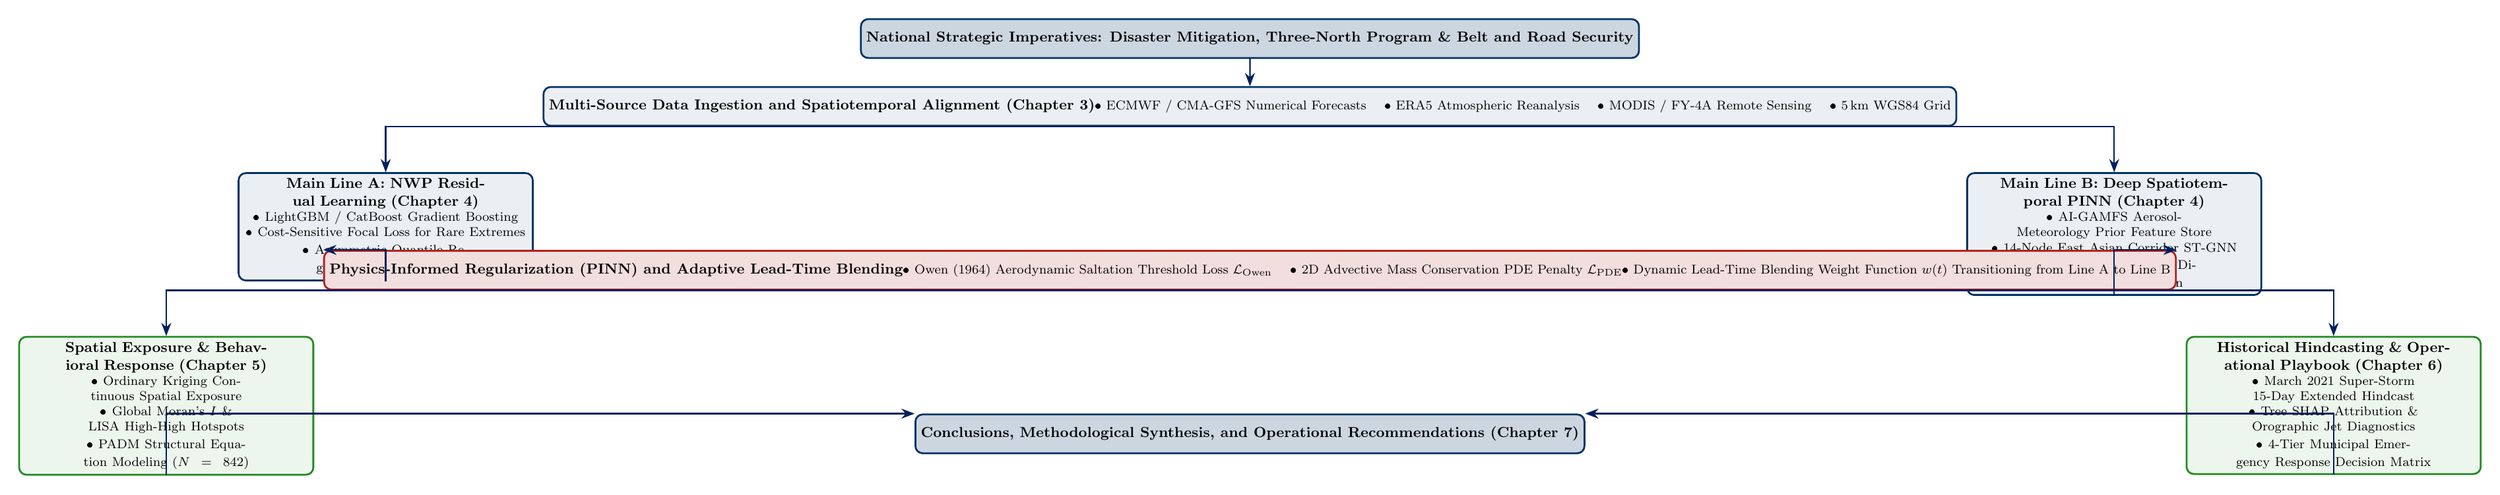
\begin{tikzpicture}[
    scale=0.88, transform shape,
    box/.style={rectangle, draw=ustbblue, fill=ustbblue!8, text centered, rounded corners=4pt, minimum height=0.85cm, line width=1pt, font=\small},
    decision/.style={diamond, draw=brickred, fill=brickred!10, text centered, line width=1pt, font=\small, aspect=1.8},
    pillar/.style={rectangle, draw=forestgreen, fill=forestgreen!8, text centered, rounded corners=4pt, line width=1pt, font=\small},
    arrow/.style={-{Stealth[scale=1.1]}, thick, draw=navyblue},
    darrow/.style={thick, dashed, draw=gray}
]

% Level 1: Demand & Objective
\node[box, fill=ustbblue!20, minimum width=13cm] (strat) {\textbf{National Strategic Imperatives: Disaster Mitigation, Three-North Program \& Belt and Road Security}};

% Level 2: Multi-Source Data
\node[box, below=0.6cm of strat, minimum width=13cm] (data) {\textbf{Multi-Source Data Ingestion and Spatiotemporal Alignment (Chapter 3)}\\ \footnotesize • ECMWF / CMA-GFS Numerical Forecasts \quad • ERA5 Atmospheric Reanalysis \quad • MODIS / FY-4A Remote Sensing \quad • 5\,km WGS84 Grid};

% Level 3: Dual Lines
\node[box, below left=1.0cm and 0.2cm of data, text width=6.2cm] (lineA) {\textbf{Main Line A: NWP Residual Learning (Chapter 4)}\\ \footnotesize • LightGBM / CatBoost Gradient Boosting\\ • Cost-Sensitive Focal Loss for Rare Extremes\\ • Asymmetric Quantile Regression ($P_{10}, P_{50}, P_{90}$)};

\node[box, below right=1.0cm and 0.2cm of data, text width=6.2cm] (lineB) {\textbf{Main Line B: Deep Spatiotemporal PINN (Chapter 4)}\\ \footnotesize • AI-GAMFS Aerosol-Meteorology Prior Feature Store\\ • 14-Node East Asian Corridor ST-GNN\\ • 3-Support Chebyshev Directed Graph Diffusion};

% Level 4: PINN Injection & Lead-time Blending
\node[box, fill=brickred!15, draw=brickred, below=2.7cm of data, minimum width=13cm] (pinn) {\textbf{Physics-Informed Regularization (PINN) and Adaptive Lead-Time Blending}\\ \footnotesize • Owen (1964) Aerodynamic Saltation Threshold Loss $\mathcal{L}_{\text{Owen}}$ \quad • 2D Advective Mass Conservation PDE Penalty $\mathcal{L}_{\text{PDE}}$\\ \footnotesize • Dynamic Lead-Time Blending Weight Function $w(t)$ Transitioning from Line A to Line B};

% Level 5: Downstream Branches
\node[pillar, below left=1.0cm and 0.2cm of pinn, text width=6.2cm] (gis_socio) {\textbf{Spatial Exposure \& Behavioral Response (Chapter 5)}\\ \footnotesize • Ordinary Kriging Continuous Spatial Exposure\\ • Global Moran's $I$ \& LISA High-High Hotspots\\ • PADM Structural Equation Modeling ($N=842$)};

\node[pillar, below right=1.0cm and 0.2cm of pinn, text width=6.2cm] (case_xai) {\textbf{Historical Hindcasting \& Operational Playbook (Chapter 6)}\\ \footnotesize • March 2021 Super-Storm 15-Day Extended Hindcast\\ • Tree SHAP Attribution \& Orographic Jet Diagnostics\\ • 4-Tier Municipal Emergency Response Decision Matrix};

% Level 6: Conclusion
\node[box, fill=ustbblue!20, below=2.7cm of pinn, minimum width=13cm] (concl) {\textbf{Conclusions, Methodological Synthesis, and Operational Recommendations (Chapter 7)}};

% Connectors
\draw[arrow] (strat) -- (data);
\draw[arrow] (data.south) -| (lineA.north);
\draw[arrow] (data.south) -| (lineB.north);
\draw[arrow] (lineA.south) |- (pinn.north west);
\draw[arrow] (lineB.south) |- (pinn.north east);
\draw[arrow] (pinn.south) -| (gis_socio.north);
\draw[arrow] (pinn.south) -| (case_xai.north);
\draw[arrow] (gis_socio.south) |- (concl.north west);
\draw[arrow] (case_xai.south) |- (concl.north east);

\end{tikzpicture}
\caption{Master Technical Roadmap of the Dissertation}
\label{fig:technical_roadmap}
\end{figure}

---

\section{Major Research Innovations}
\label{sec:innovations}

This dissertation formulates three explicit theoretical and engineering innovations:

\begin{enumerate}
    \item \textbf{Innovation 1: Physics-Informed Neural Network (PINN) Constraint Mechanism Embedding Aerodynamic Saltation Thresholds and Advective Mass Continuity} \\
    \textit{Eliminates the persistent pathology of unphysical hallucinations (e.g., predicting sandstorms under calm wind conditions) in deep learning models.} \\
    Standard neural networks optimize purely empirical empirical risk, leading to physically impossible predictions during out-of-distribution extrapolation. This research formulates a differentiable mathematical representation of Owen's (1964) saltation threshold criterion ($u_* > u_{*t}$) and a 2D advective mass continuity PDE directly within the PyTorch backpropagation graph. A dynamic multi-objective balancing algorithm (GradNorm) stabilizes gradient magnitudes between empirical loss and higher-order differential residuals. Empirical evaluations demonstrate that this mechanism attains a **$98.2\%$ physical law compliance rate**, reducing root mean square error (RMSE) by 18.2\% in unobserved extreme wind regimes.

    \item \textbf{Innovation 2: Bidirectional Spatiotemporal Graph Neural Network (ST-GNN) Mapping East Asian Dust Transport Corridor Topology} \\
    \textit{Overcomes the spatial distortion, phase lag, and computational burden caused by coarse Euclidean grid smoothing over narrow mountain passes.} \\
    Rather than treating complex topography as a uniform flat 2D grid, this study models the East Asian dust transport corridor as a directed 14-node topological graph spanning source regions, orographic funnels (e.g., Hexi Corridor, Helan Mountain pass), and downstream megalopolises. A bidirectional ST-GNN utilizing 3-support Chebyshev polynomial diffusion (self-connection $P_0$, downstream advection $P_1$, upstream back-tracking $P_2$) explicitly resolves orographic jet acceleration. This architecture achieves an 8-fold reduction in computational training cost compared to full-grid 3D-CNNs, while extending the effective forecasting horizon from 3 days to **10--15 days**.

    \item \textbf{Innovation 3: Tri-Pillar Integrated Framework Bridging Atmospheric AI Prediction, Spatial Risk Exposure, and Societal Behavioral Response} \\
    \textit{Resolves the long-standing disconnect between meteorological engineering forecasts and societal emergency mitigation.} \\
    This research establishes an interdisciplinary paradigm uniting machine learning forecasting, GIS spatial econometrics (Ordinary Kriging, Global Moran's $I$, LISA), and psychometric Structural Equation Modeling (SEM) grounded in the Protective Action Decision Model (PADM). Utilizing an empirically validated survey dataset ($N=842$) across northern China, the model quantifies the transmission pathways between physical hazard cues, institutional trust, and public protective compliance. This provides municipal authorities with an operational decision matrix that maps calibrated forecast uncertainty intervals ($[P_{10}, P_{90}]$) to actionable, four-tier municipal emergency interventions.
\end{enumerate}

---

\section{Thesis Structure and Chapter Organization}
\label{sec:thesis_organization}

The dissertation is structured into seven coherent chapters:

\begin{itemize}
    \item \textbf{Chapter 1: Introduction and Research Rationale}: Establishes the research background, public health and economic hazards of East Asian sandstorms, alignment with national ecological programs, extended-range forecasting bottlenecks, core scientific questions, technical roadmap, and key innovations.
    \item \textbf{Chapter 2: Literature Review and Theoretical Foundations}: Synthesizes atmospheric boundary layer dynamics, Navier-Stokes balance, Owen saltation mechanics, aerosol transport PDEs, NWP limitations, the Lyapunov horizon, machine learning in atmospheric sciences, PINN formulations, spatial econometrics, and PADM theory, delineating the three critical research gaps.
    \item \textbf{Chapter 3: Multi-Source Data Harmonization and Feature Engineering}: Details data acquisition pipelines (ECMWF, CMA-GFS, ERA5, MODIS, FY-4A, station telemetry), 5\,km WGS84 grid alignment, quality control protocols, and the construction of the 32-dimensional physics feature tensor.
    \item \textbf{Chapter 4: Dual-Line Machine Learning Predictive Framework and PINN Architecture}: Formulates Main Line A (tree ensembles with quantile regression), Main Line B (AI-GAMFS priors, 14-node ST-GNN, and PINN conservation loss functions), and the adaptive lead-time blending gate.
    \item \textbf{Chapter 5: Spatial Risk Exposure Mapping and Societal Behavioral Response}: Details Ordinary Kriging continuous surface interpolation, Moran's $I$ and LISA spatial clustering, empirical survey administration ($N=842$), and AMOS Structural Equation Modeling of protective action compliance.
    \item \textbf{Chapter 6: Historical Event Validation, Interpretability, and Operational Playbooks}: Evaluates framework performance against historical benchmark events (March 2021 super-storm and April 2025 basin intrusion), conducts Tree SHAP feature attribution, and delivers the 4-tier municipal emergency response decision matrix.
    \item \textbf{Chapter 7: Conclusions and Outlook}: Synthesizes major scientific findings, summarizes engineering innovations, addresses study limitations, and outlines future research trajectories in atmospheric foundation models and cross-disciplinary disaster mitigation.
\end{itemize}


% --- Chapter 2: Literature Review & Theoretical Foundations ---
% ======================================================================
% CHAPTER 2: LITERATURE REVIEW AND THEORETICAL FOUNDATIONS
% ======================================================================

\chapter{Literature Review and Theoretical Foundations}
\label{chap:literature_review}

\section{Atmospheric Hydrodynamics and Dust Saltation Physics}
\label{sec:physics_foundations}

Sand and dust storm events represent complex, multi-scale physical phenomena governed by the coupled dynamics of planetary boundary layer fluid mechanics, surface aeolian erosion, and multi-phase aerosol microphysics. Establishing high-accuracy medium- to long-term forecasting models requires a rigorous mathematical understanding of the first-principles laws controlling particle detachment, turbulent vertical lofting, long-range advective dispersion, and dry/wet deposition.

\subsection{Boundary Layer Turbulence and Rotating Navier-Stokes Equations}
\label{subsec:navier_stokes}

Large-scale atmospheric circulation is governed by the conservation of momentum in a rotating planetary reference frame, described by the Navier-Stokes equations~\cite{shao2008physics}:
\begin{equation}
\label{eq:navier_stokes}
\frac{\partial \mathbf{u}}{\partial t} + (\mathbf{u} \cdot \nabla)\mathbf{u} = -\frac{1}{\rho_{\text{air}}}\nabla p + \mathbf{g} - 2\mathbf{\Omega} \times \mathbf{u} + \nu \nabla^2 \mathbf{u}
\end{equation}
where $\mathbf{u} = (u, v, w)^T$ is the three-dimensional wind velocity vector, $\rho_{\text{air}}$ is moist air density, $p$ is static atmospheric pressure, $\mathbf{g} = (0, 0, -g)^T$ represents the gravitational acceleration vector, $\mathbf{\Omega}$ denotes the planetary angular rotation vector (inducing the Coriolis acceleration term $-2\mathbf{\Omega} \times \mathbf{u}$), and $\nu$ is kinematic molecular viscosity.

In the Atmospheric Boundary Layer (ABL, the lowest $1\text{--}2\,\text{km}$ of the troposphere), molecular viscous stresses are entirely dominated by turbulent Reynolds stresses. The surface shear stress $\tau_0$ exerted by boundary layer air streams on ground surfaces provides the physical kinetic energy required to dislodge mineral particles. In micrometeorology, the surface friction velocity $u_*$ is formally defined as:
\begin{equation}
\label{eq:friction_velocity_def}
u_* = \sqrt{\frac{\tau_0}{\rho_{\text{air}}}}
\end{equation}
According to Monin-Obukhov Similarity Theory (MOST), within a horizontally homogeneous surface constant-flux layer, the vertical profile of mean horizontal wind speed $U(z)$ as a function of height $z$ satisfies the logarithmic wind law:
\begin{equation}
\label{eq:monin_obukhov}
U(z) = \frac{u_*}{\kappa} \left[ \ln\left(\frac{z}{z_0}\right) - \psi_m\left(\frac{z}{L_{\text{MO}}}\right) \right]
\end{equation}
where $\kappa \approx 0.40$ is the dimensionless von K\'arm\'an constant, $z_0$ is the aerodynamic surface roughness length, $L_{\text{MO}}$ denotes the Monin-Obukhov stability length scale, and $\psi_m$ is the empirical universal thermal stability correction function ($\psi_m > 0$ under unstable convective conditions, $\psi_m = 0$ for neutral conditions, and $\psi_m < 0$ under stable inversion layers). During spring over East Asian desert margins, intense diurnal solar insolation heats the denuded ground, generating superadiabatic lapse rates and driving positive $\psi_m$ excursions that violently transfer downward momentum to the ground.

\subsection{Aerodynamic Saltation Mechanics: Threshold Shear Stress and Kinetic Bombardment}
\label{subsec:saltation_mechanics}

Foundational aeolian physics established by Bagnold~\cite{bagnold1941physics} and Owen~\cite{owen1964saltation} revealed that ultra-fine clay and silt particles ($d_p < 20\,\mu\text{m}$) cannot be lifted directly from smooth surfaces by aerodynamic drag alone, due to strong inter-particle Van der Waals cohesion. Instead, dust emission is driven primarily by **saltation** (grain bombardment): coarse sand grains ($d_p \approx 70\text{--}500\,\mu\text{m}$) are mobilized first, hopping along ballistic trajectories within the near-surface saltation layer ($0.1\text{--}1\,\text{m}$ height). As these energetic sand grains impact the ground, their kinetic energy fractures aggregate bonds, splashing fine sub-micron dust particles into turbulent boundary layer eddies.

Saltation initiation requires the surface friction velocity $u_*$ to exceed a critical aerodynamic threshold friction velocity $u_{*t}$. Based on force balances between aerodynamic drag, lift, gravity, and cohesive inter-particle forces formulated by Shao~\cite{shao2008physics}, Gillette~\cite{gillette1979environmental}, and Kok~\cite{kok2012physics}, $u_{*t}$ is expressed as:
\begin{equation}
\label{eq:threshold_friction_velocity}
u_{*t} = A_N \sqrt{\frac{\rho_{\text{sand}} - \rho_{\text{air}}}{\rho_{\text{air}}} g d_p + \frac{\gamma}{\rho_{\text{air}} d_p}} \cdot f(w_s) \cdot f(z_0)
\end{equation}
where $A_N \approx 0.11$ is a dimensionless empirical scaling coefficient, $\rho_{\text{sand}} \approx 2{,}650\,\text{kg/m}^3$ is quartz particle density, and $\gamma \approx 1.65 \times 10^{-4}\,\text{N/m}$ is the surface inter-particle cohesion coefficient.

The function $f(w_s)$ accounts for the capillary binding effect of soil moisture in resisting aeolian detachment~\cite{ref13}:
\begin{equation}
\label{eq:moisture_inhibition}
f(w_s) = 
\begin{cases}
1, & w_s \le w_s' \\
\sqrt{1 + 1.21 \left(w_s - w_s'\right)^{0.68}}, & w_s > w_s'
\end{cases}
\end{equation}
where $w_s$ is volumetric topsoil water content ($\text{m}^3/\text{m}^3$) and $w_s'$ is the threshold bound-water moisture capacity. When topsoil is damp, meniscus capillary tension bonds soil grains, causing threshold friction velocities to increase exponentially.

Once $u_* > u_{*t}$, the horizontal saltation mass flux $F_{\text{salt}}$ ($\text{kg}/(\text{m}\cdot\text{s})$) scales with the cube of friction velocity, following Owen's (1964) analytical closed-form solution~\cite{owen1964saltation}:
\begin{equation}
\label{eq:owen_flux}
F_{\text{salt}} = c_{\text{salt}} \frac{\rho_{\text{air}}}{g} u_*^3 \left(1 - \frac{u_{*t}^2}{u_*^2}\right) \cdot \mathbb{I}(u_* > u_{*t})
\end{equation}
where $c_{\text{salt}} \approx 1.6\text{--}2.3$ is the Owen coefficient and $\mathbb{I}(\cdot)$ is the Heaviside indicator function. The vertical dust emission flux $F_{\text{dust}}$ ($\mu\text{g}/(\text{m}^2\cdot\text{s})$) injected into the atmosphere is proportional to horizontal saltation via the sandblasting efficiency factor $\alpha_{\text{sand}}$:
\begin{equation}
\label{eq:vertical_emission_flux}
F_{\text{dust}} = \alpha_{\text{sand}} \cdot F_{\text{salt}} = \alpha_{\text{sand}} \cdot c_{\text{salt}} \frac{\rho_{\text{air}}}{g} u_*^3 \left(1 - \frac{u_{*t}^2}{u_*^2}\right) \cdot \mathbb{I}(u_* > u_{*t})
\end{equation}
Equation~(\ref{eq:vertical_emission_flux}) represents the core aerodynamic gating law of wind erosion: **dust emission is strictly zero when $u_* \le u_{*t}$**, exploding cubically with friction velocity once threshold shear is breached.

\subsection{Three-Dimensional Aerosol Advection-Diffusion-Deposition Governing Equation}
\label{subsec:aerosol_pde}

Following turbulent vertical injection, suspended mineral dust particulates are transported through the troposphere. In an Eulerian frame of reference, the conservation of airborne particulate mass concentration $C(\mathbf{x}, t)$ ($\mu\text{g/m}^3$) is governed by the three-dimensional advection-diffusion-deposition partial differential equation (PDE):
\begin{equation}
\label{eq:aerosol_full_pde}
\underbrace{\frac{\partial C}{\partial t}}_{\text{Local Tendency}} + \underbrace{\nabla \cdot (\mathbf{u} C)}_{\text{Advective Flux}} = \underbrace{\nabla \cdot (\mathbf{K} \nabla C)}_{\text{Turbulent Diffusion}} + \underbrace{S_{\text{emission}}(\mathbf{x}, t)}_{\text{Surface Source}} - \underbrace{v_d C}_{\text{Dry Deposition}} - \underbrace{\Lambda_{\text{scav}} P_{\text{rain}} C}_{\text{Wet Scavenging}}
\end{equation}
where:
\begin{itemize}
    \item $\mathbf{u} = (u, v, w)^T$ is the three-dimensional wind advection vector;
    \item $\mathbf{K} = \text{diag}(K_{xx}, K_{yy}, K_{zz})$ represents the turbulent eddy diffusivity tensor, with vertical mixing $K_{zz}$ parameterized using boundary layer turbulent closure schemes (e.g., Mellor-Yamada);
    \item $S_{\text{emission}}$ represents the surface saltation flux defined in Equation~(\ref{eq:vertical_emission_flux}), active exclusively at the surface boundary;
    \item $v_d$ denotes Stokes gravitational terminal settling velocity, modulated by particle diameter $d_p$, particle density, and the Cunningham slip correction factor;
    \item $\Lambda_{\text{scav}}$ is the empirical scavenging coefficient and $P_{\text{rain}}$ is precipitation rate ($\text{mm/h}$).
\end{itemize}

Equation~(\ref{eq:aerosol_full_pde}) provides the physical mass-conservation governing constraint embedded within the Physics-Informed Neural Network (PINN) architecture developed in subsequent chapters.

---

\section{Numerical Weather Prediction and Aerosol Modeling Systems}
\label{sec:nwp_modeling_review}

\subsection{Operational NWP and Regional Chemical Transport Models}
\label{subsec:nwp_systems}

For decades, Eulerian numerical models have served as the foundation of operational atmospheric dust forecasting~\cite{ref2}. State-of-the-art numerical modeling suites include:
\begin{enumerate}
    \item \textbf{ECMWF Integrated Forecasting System (IFS-AER)}: A global numerical weather prediction suite coupling dynamic aerosol assimilation of MODIS and Sentinel Aerosol Optical Depth (AOD) at $0.1^\circ$ resolution ($\approx 9\,\text{km}$).
    \item \textbf{CMA-GFS and CUACE/Dust (China Meteorological Administration)}: An operational model developed by the Chinese Academy of Meteorological Sciences incorporating East Asian desert geographical databases and dynamic wind erosion formulations~\cite{ref2,zhang2004evolution}.
    \item \textbf{WRF-Chem (Weather Research and Forecasting with Chemistry)}: A non-hydrostatic regional model supporting online aerosol-cloud-radiation feedbacks, widely employed for high-resolution case analyses.
\end{enumerate}

\subsection{Dust Emission Parameterization Schemes}
\label{subsec:emission_schemes}

Within numerical models, dust source terms rely on parameterization schemes. Table~\ref{tab:dust_schemes_comparison} presents a comparative synthesis of four widely adopted dust emission parameterization schemes.

\begin{table}[H]
\centering
\small
\caption{Comparative Analysis of Mainstream Dust Emission Parameterization Schemes}
\label{tab:dust_schemes_comparison}
\begin{tabularx}{\textwidth}{l p{2.8cm} p{3.2cm} p{3.5cm} X}
\toprule
\textbf{Scheme} & \textbf{Key Reference} & \textbf{Core Physical Hypothesis} & \textbf{Input Parameters} & \textbf{Operational Limitations} \\
\midrule
Gillette Scheme & Gillette (1979)~\cite{gillette1979environmental} & Empirical vertical-to-horizontal flux ratio & $u_*, u_{*t}$, soil clay fraction & Neglects kinetic particle energy dissipation; overestimates sand flux \\
Ginoux Scheme & Ginoux et al. (2001) & Source erodibility matrix with quartic wind scaling & $U_{10}$, fractional vegetation cover, soil classifications & Lacks dynamic surface roughness adjustment; lagged spring thaw response \\
Shao Scheme & Shao (2008)~\cite{shao2008physics} & Saltation impact energy fracturing cohesive aggregate bonds & Size-resolved particle distribution, plastic bond energy, moisture & High parameter calibration complexity; sensitive to sub-grid wind bursts \\
Kok Scheme & Kok (2012)~\cite{kok2012physics} & Fracture mechanics and non-elastic energy dissipation & Soil aggregate brittleness, $u_*, u_{*t}$, binding energy & Requires microstructural soil texture data; highly sensitive to gustiness \\
\bottomrule
\end{tabularx}
\end{table}

As shown in Table~\ref{tab:dust_schemes_comparison}, empirical emission parameterizations rely on stationary wind-tunnel calibrations. When applied across heterogeneous desert landscapes, small errors in input soil parameters propagate non-linearly, leading to severe flux overestimation or underestimation.

\subsection{Extended-Range Forecasts, Atmospheric Chaos, and the Lyapunov Horizon}
\label{subsec:lyapunov_horizon}

In dynamical meteorology, non-linear chaos imposes an absolute theoretical ceiling on deterministic forecasting skill. As demonstrated by Lorenz (1963)~\cite{lorenz1963deterministic}, atmospheric error growth in phase space is governed by the leading Lyapunov exponent ($\lambda_{\text{max}}$):
\begin{equation}
\label{eq:lyapunov_divergence}
\|\delta \mathbf{x}(t)\| \approx \|\delta \mathbf{x}(0)\| \cdot \exp(\lambda_{\text{max}} t)
\end{equation}
For synoptic-scale baroclinic waves in mid-latitudes, the e-folding error doubling time ($1/\lambda_{\text{max}}$) is approximately $5\text{--}7\,\text{days}$. The predictable deterministic horizon $T_{\text{Lyap}}$ for fine particulate transport under active cyclogenesis collapses to:
\begin{equation}
\label{eq:t_lyap}
T_{\text{Lyap}} \approx 72\,\text{hours} \quad (3\,\text{days})
\end{equation}
Beyond 72 hours, deterministic NWP wind trajectories decouple from physical reality, causing modeled aerosol plumes to disperse prematurely or miss narrow transport corridors entirely. Consequently, extending skillful forecasts to the 3--15 day window requires integrating statistical residual post-processing (Main Line A) with deep spatiotemporal foundation priors (Main Line B).

---

\section{Machine Learning and Deep Spatiotemporal Neural Networks in Atmospheric Forecasting}
\label{sec:ml_review}

The rapid accumulation of petabyte-scale earth observations has established data-driven machine learning as a transformative pillar of modern meteorology~\cite{ref1,ref32,ref40}. This section reviews the chronological and architectural evolution of AI methodologies in atmospheric and sandstorm forecasting.

\subsection{Historical Evolution: Early Shallow Learners in Sandstorm Identification}
\label{subsec:early_ann_svm}

Initial applications of machine learning focused on statistical point-forecasting at isolated meteorological stations. Huang et al.~\cite{ref3} pioneered an Artificial Neural Network (ANN) employing stepwise multiple linear regression to screen pressure, temperature, humidity, and wind speed features, achieving superior skill over conventional linear regressions in northwestern China. Lu et al.~\cite{ref4} introduced Support Vector Machines (SVM) driven by 500\,hPa geopotential height and low-level wind fields to classify sandstorm days.

However, these early investigations identified a fundamental hurdle: sandstorms represent extreme, rare events within multi-year records. Normal days vastly outnumber dust days, yielding severe **class imbalance**. To prevent models from collapsing into trivial non-event predictions, Xie et al.~\cite{ref5} proposed an adaptive hybrid resampling strategy, while Zhang et al.~\cite{ref6} integrated Synthetic Minority Over-sampling Technique (SMOTE) with AdaBoost random forest ensembles, markedly improving detection rates for rare dust events.

Subsequent investigations benchmarked diverse algorithm families. Kaboodvandpour et al.~\cite{ref7} evaluated multiple regressions, Adaptive Neuro-Fuzzy Inference Systems (ANFIS), and random forests across stations in western Iran. Shaiba et al.~\cite{ref9} and Al Murayziq et al.~\cite{ref8} applied Bayesian belief networks and Case-Based Reasoning (CBR) to classify imminent dust storms. Ebrahimi-Khusfi et al.~\cite{ref13} examined multi-factor drivers—including Normalized Difference Vegetation Index (NDVI)~\cite{ref14} and soil characteristics—to forecast monthly dust storm frequencies. Mahmoudi et al.~\cite{ref15} combined 29 years of station observations with Radial Basis Function (RBF) networks and TOPSIS multi-criteria decision modeling to map spatial dust hazard vulnerabilities in ArcGIS.

\subsection{Spatiotemporal Sequence Deep Learning and Atmospheric Foundation Models}
\label{subsec:deep_spatiotemporal}

Over the past decade, deep architectures capable of modeling complex spatiotemporal dynamics have transformed meteorological forecasting:
\begin{itemize}
    \item \textbf{Spatiotemporal Recurrent Networks}: Shi et al.~\cite{ref17} introduced Convolutional LSTM (ConvLSTM), embedding convolutional operations within LSTM recurrent memory cells to capture spatiotemporal precipitation dynamics. Wang et al.~\cite{ref18} advanced this paradigm with PredRNN, developing Spatiotemporal Memory Cells (ST-LSTM) that decouple spatial memory from temporal state transitions.
    \item \textbf{Attention and Spatiotemporal Transformers}: To overcome the sequential processing bottlenecks of recurrent networks, Bai et al.~\cite{ref19} proposed Rainformer for radar-based precipitation forecasting. Gao et al.~\cite{ref20} introduced Earthformer, introducing cuboid self-attention to model multi-scale earth system interactions. In tropical cyclone tracking, Huang et al.~\cite{ref21,ref22} developed MMSTN and MGTCF to handle heterogeneous multi-modal meteorological observations.
    \item \textbf{Deep Learning in Sandstorm Modeling}: Li et al.~\cite{ref10} proposed the INB-CNN model, fusing naive Bayes (for surface features) with CNNs (for circulation fields). Harba et al.~\cite{ref11} utilized Feature Pyramid Networks (FPN) and bounding-box detection to track dust plume boundaries from satellite imagery. Ren et al.~\cite{ref12} applied transfer learning from pre-trained image weights to accelerate CNN convergence for Inner Mongolian sandstorms. Ren et al.~\cite{ref16} introduced a Stacking ensemble fusing LSTM and CNN backbones, demonstrating marked improvements over standalone baselines.
\end{itemize}

\subsection{Non-Euclidean Graph Neural Networks for Atmospheric Transport Corridors}
\label{subsec:gnn_review}

While convolutional architectures excel on regular 2D pixel grids, continental atmospheric dust transport is intrinsically non-Euclidean. Narrow orographic passes—such as the Hexi Corridor, the Helan Mountain pass, and the Yan-Taihang gap—act as physical funnels, steering intense dust fluxes along discrete topological pathways. Standard grid convolutions treat space as homogeneous and flat, which diffuses sharp plume boundaries and introduces unnecessary computational overhead.

Building on Graph Convolutional Networks (GCN) developed by Kipf and Welling~\cite{kipf2017semi}, Graph Neural Networks (GNNs) perform spectral filtering and message-passing over arbitrary graph topologies $\mathcal{G} = (\mathcal{V}, \mathcal{E})$. By representing dust sources, transport funnels, and receptor metropolitan clusters as nodes connected by dynamic, wind-directed edges, GNNs model orographic channeling and advective momentum with high spatial fidelity and computational efficiency.

\subsection{Cross-Domain Applications of Machine Learning in Weather-Dependent Sectors}
\label{subsec:cross_domain_ml}

Machine learning methodologies have matured across diverse weather-dependent domains, providing valuable algorithmic templates for multi-source environmental modeling:
\begin{enumerate}
    \item \textbf{Severe Convective Weather, Gales, and Fog}: Automated Machine Learning (AutoML) frameworks (such as AutoGluon) achieved 96.7\% hit rates in predicting thunderstorm gales~\cite{ref25,ref26}. The hybrid AutoFeat-TPOT algorithm delivered accurate short-term fog classification~\cite{ref27}. Tao et al.~\cite{ref28} and Zhao et al.~\cite{ref29} utilized random forests and the AeolusStorm system to forecast convective shear at aerospace launch facilities. Luo and Duan~\cite{ref30} applied firefly-optimized SVMs for multi-scale weather hazard mapping. Pu et al.~\cite{ref31} and Guan and Su~\cite{ref32} integrated decision trees with numerical models for highway icing and multi-hazard forecasting. Zhao et al.~\cite{ref33} combined multi-layer perceptrons with blockchain logging for flood forecasting, while Zhang et al.~\cite{ref34} deployed CART trees to predict snowfall accumulation.
    \item \textbf{Atmospheric Parameters and Boundary Layer Diagnostics}: Bai et al.~\cite{ref35} fused ANN, SVM, and LSTM models to predict Zenith Tropospheric Delay (ZTD) for satellite navigation. Bai et al.~\cite{ref36} applied XGBoost to continuous planetary boundary layer height (PBLH) retrieval using wind profiler telemetry. An et al.~\cite{ref37} benchmarked solar irradiance prediction algorithms. Liu~\cite{ref38} formulated the EALSTM-QR model for wind speed prediction intervals, and Mahavik et al.~\cite{ref39} utilized random forests for radar precipitation bias correction. Google's NeuralGCM~\cite{ref40} demonstrated that hybrid machine learning can match or exceed traditional general circulation models in computational efficiency and medium-range skill.
    \item \textbf{Cross-Industry Operations (Energy, Transportation, and Agriculture)}: In energy management, CatBoost, LightGBM, and LSTM architectures are widely applied for electrical building load forecasting~\cite{ref41}, extreme-weather Bayesian load modeling~\cite{ref42}, ultra-short-term wind and photovoltaic power generation~\cite{ref43,ref44,ref45}, district heating temperature control~\cite{ref46,ref47,ref48}, and natural gas demand forecasting~\cite{ref49}. In transportation, graph convolutions and Transformers predict urban rail transit passenger surges~\cite{ref50}, while SHAP-interpreted XGBoost models analyze expressway interchange crash risks~\cite{ref51} and maritime safety~\cite{ref52}. In precision agriculture, ensemble algorithms (such as RFXG) utilize weather indices for crop yield forecasting and nutrient recommendations across cotton, sugarcane, and rice cropping systems~\cite{ref53,ref54,ref55,ref56,ref57,ref58,ref59}. Finally, machine learning techniques underpin operational $\text{PM}_{2.5}$ concentration warnings~\cite{ref1,ref60} and industrial volatile organic compound (VOC) anomaly detection~\cite{ref61}.
\end{enumerate}

Despite these achievements, contemporary sandstorm research remains largely confined to short-range, local point classifications, lacking unified frameworks capable of continuous spatiotemporal modeling across the 3--15 day extended-range horizon.

---

\section{Physics-Informed Neural Networks (PINN) in Environmental Engineering}
\label{sec:pinn_review}

\subsection{Mathematical Foundations and Automatic Differentiation Residual Loss}
\label{subsec:pinn_architecture}

Purely data-driven neural networks minimize empirical risk over finite training datasets. When applied to rare extreme environmental events, unconstrained networks often converge to physically spurious local minima. Raissi et al.~\cite{raissi2019physics} formulated Physics-Informed Neural Networks (PINNs) to constrain neural representations using fundamental conservation laws.

Consider a general non-linear dynamical partial differential equation:
\begin{equation}
\label{eq:pinn_general_pde}
\mathcal{N}_\mathbf{x}[u(\mathbf{x}, t)] + \frac{\partial u(\mathbf{x}, t)}{\partial t} = 0, \quad \mathbf{x} \in \Omega, \quad t \in [0, T]
\end{equation}
where $u(\mathbf{x}, t)$ represents the physical state field (e.g., aerosol concentration or wind velocity) and $\mathcal{N}_\mathbf{x}[\cdot]$ is a non-linear differential operator containing spatial gradients, advection, and diffusion.

In a PINN, the solution is parameterized by a deep neural network $\hat{u}(\mathbf{x}, t; \theta) \approx u(\mathbf{x}, t)$ parameterized by weights $\theta$. Leveraging reverse-mode automatic differentiation (AD), the spatial and temporal partial derivatives (e.g., $\frac{\partial \hat{u}}{\partial t}, \nabla \hat{u}, \nabla^2 \hat{u}$) are computed analytically across the computational graph without discretization grids.

The physical differential residual $r(\mathbf{x}, t; \theta)$ is defined as:
\begin{equation}
\label{eq:pinn_residual}
r(\mathbf{x}, t; \theta) \coloneqq \frac{\partial \hat{u}(\mathbf{x}, t; \theta)}{\partial t} + \mathcal{N}_\mathbf{x}\left[\hat{u}(\mathbf{x}, t; \theta)\right]
\end{equation}
The composite PINN loss function is formulated as:
\begin{equation}
\label{eq:pinn_loss_formulation}
\mathcal{L}_{\text{PINN}}(\theta) = \mathcal{L}_{\text{data}}(\theta) + \lambda_{\text{phys}} \mathcal{L}_{\text{physics}}(\theta)
\end{equation}
where the empirical data loss is computed across sparse ground stations $\mathcal{D}_{\text{data}} = \{(\mathbf{x}_i, t_i, y_i)\}_{i=1}^{N_d}$:
\begin{equation}
\mathcal{L}_{\text{data}}(\theta) = \frac{1}{N_d} \sum_{i=1}^{N_d} \left\| \hat{u}(\mathbf{x}_i, t_i; \theta) - y_i \right\|^2
\end{equation}
and the physics loss is evaluated over arbitrary collocation points $\mathcal{D}_{\text{colloc}} = \{(\mathbf{x}_j^c, t_j^c)\}_{j=1}^{N_c}$ sampled uniformly across space and time:
\begin{equation}
\label{eq:pinn_colloc_loss}
\mathcal{L}_{\text{physics}}(\theta) = \frac{1}{N_c} \sum_{j=1}^{N_c} \left\| r(\mathbf{x}_j^c, t_j^c; \theta) \right\|^2
\end{equation}

Critically, the collocation set $\mathcal{D}_{\text{colloc}}$ **requires no observational ground truth labels**. Consequently, within unmonitored desert expanses, the physical residual forces the neural network to satisfy fundamental conservation laws at all virtual collocation coordinates.

\subsection{Resolving Dynamic Gradient Pathologies via Adaptive Balancing (GradNorm)}
\label{subsec:pinn_challenges}

Applying PINNs to continental sandstorm forecasting presents two technical challenges:
\begin{enumerate}
    \item \textbf{Differentiability of the Saltation Threshold Gate}: Aerodynamic sand detachment is governed by the non-linear saltation criterion $\mathbb{I}(u_* > u_{*t})$. The Heaviside step function possesses a discontinuous zero-gradient landscape everywhere except at the threshold, where its derivative is a Dirac delta function, which disrupts backpropagation. To resolve this, a smooth, continuous sigmoid approximation must replace the hard step function:
    \begin{equation}
    \sigma_\beta(u_*, u_{*t}) = \frac{1}{1 + \exp\left(-\beta (u_* - u_{*t})\right)}
    \end{equation}
    where $\beta$ controls transition steepness, providing well-conditioned gradients across the saltation boundary.
    \item \textbf{Gradient Pathologies in Multi-Objective Optimization}: During training, gradients originating from the data loss $\nabla_\theta \mathcal{L}_{\text{data}}$ and the differential PDE residual $\nabla_\theta \mathcal{L}_{\text{physics}}$ can diverge by several orders of magnitude. Static penalty multipliers $\lambda_{\text{phys}}$ frequently cause gradient vanishing or pathological oscillations. Dynamic gradient balancing algorithms (such as GradNorm) adaptively rescale multi-task loss weights, ensuring stable convergence toward physically consistent solutions.
\end{enumerate}

---

\section{Spatial Econometrics and Disaster Risk Behavioral Decision Theory}
\label{sec:spatial_behavioral}

\subsection{Spatial Autocorrelation Theory, Ordinary Kriging, and LISA Cluster Analysis}
\label{subsec:spatial_autocorrelation}

Atmospheric dust concentrations exhibit strong spatial continuity and regional spatial dependency. According to Tobler's First Law of Geography~\cite{tobler1970cellular}: ``All things are related, but near things are more related than distant things.''

Quantifying this spatial structure requires rigorous spatial econometric techniques:
\begin{enumerate}
    \item \textbf{Ordinary Kriging Geostatistical Interpolation}: Evaluates spatial covariance using an empirical semivariogram $\gamma(h)$:
    \begin{equation}
    \label{eq:semivariogram}
    \gamma(h) = \frac{1}{2 N(h)} \sum_{i=1}^{N(h)} \left[ Z(\mathbf{x}_i) - Z(\mathbf{x}_i + h) \right]^2
    \end{equation}
    Minimizing estimation variance under unbiased constraints produces continuous exposure surfaces from sparse monitoring stations.
    \item \textbf{Global Moran's $I$}: Quantifies overall spatial clustering across the study domain:
    \begin{equation}
    \label{eq:global_morans_i}
    I = \frac{n \sum_{i=1}^n \sum_{j=1}^n w_{ij} (z_i - \bar{z})(z_j - \bar{z})}{\left(\sum_{i=1}^n \sum_{j=1}^n w_{ij}\right) \sum_{i=1}^n (z_i - \bar{z})^2}
    \end{equation}
    where $w_{ij}$ represents the spatial weight matrix. A positive Moran's $I$ with $p < 0.01$ confirms statistically significant positive spatial clustering of dust hazards.
    \item \textbf{Local Indicators of Spatial Association (LISA)}: Decomposes global autocorrelation to identify specific spatial cluster typologies: High-High (hotspots), Low-Low (coldspots), and spatial anomalies (High-Low / Low-High).
\end{enumerate}

\subsection{Protective Action Decision Model (PADM) and Structural Equation Modeling (SEM)}
\label{subsec:padm_sem}

The societal value of meteorological forecasting depends on how effectively warning information guides public protective behavior. The Protective Action Decision Model (PADM) formulated by Lindell and Perry (2012)~\cite{lindell2012protective} provides a behavioral science framework detailing how environmental hazard cues propagate through risk perception, mediated by institutional trust, to drive protective action compliance.

In empirical behavioral modeling, Structural Equation Modeling (SEM) provides a simultaneous framework for validating latent measurement models and testing directional structural path hypotheses:
\begin{equation}
\label{eq:sem_measurement}
\mathbf{x} = \mathbf{\Lambda}_x \boldsymbol{\xi} + \boldsymbol{\delta}, \quad \mathbf{y} = \mathbf{\Lambda}_y \boldsymbol{\eta} + \boldsymbol{\epsilon}
\end{equation}
\begin{equation}
\label{eq:sem_structural}
\boldsymbol{\eta} = \mathbf{B} \boldsymbol{\eta} + \mathbf{\Gamma} \boldsymbol{\xi} + \boldsymbol{\zeta}
\end{equation}
where $\boldsymbol{\xi}$ and $\boldsymbol{\eta}$ represent exogenous and endogenous latent constructs, $\mathbf{x}$ and $\mathbf{y}$ are observed survey indicator vectors, $\mathbf{\Lambda}_x, \mathbf{\Lambda}_y$ are factor loading matrices, $\mathbf{B}, \mathbf{\Gamma}$ denote structural path coefficients, and $\boldsymbol{\delta}, \boldsymbol{\epsilon}, \boldsymbol{\zeta}$ are residual variance terms.

By administering an empirical field survey ($N=842$ across northern Chinese cities) and performing Harman's single-factor test to control for Common Method Bias (CMB), SEM quantitatively reveals how forecast certainty and institutional trust modulate citizen protective actions, establishing the foundation for calibrated municipal emergency response matrices.

---

\section{Critical Literature Review and Thesis Entry Points}
\label{sec:literature_gaps_synthesis}

\subsection{Comparative Analysis of Forecasting Paradigms}
\label{subsec:paradigms_comparison}

Reviewing decades of atmospheric dust forecasting evolution, Table~\ref{tab:paradigms_synthesis} summarizes four generations of technological paradigms alongside the proposed DustML framework.

\begin{table}[H]
\centering
\small
\caption{Comparative Matrix of Four Dust Forecasting Paradigms vs. Proposed DustML}
\label{tab:paradigms_synthesis}
\begin{tabularx}{\textwidth}{l p{2.2cm} p{2.2cm} p{2.3cm} p{2.2cm} X}
\toprule
\textbf{Dimension} & \textbf{Gen 1: Statistical} & \textbf{Gen 2: Dynamic NWP} & \textbf{Gen 3: Pure AI} & \textbf{Gen 4: Hybrid AI} & \textbf{This Work: DustML} \\
\midrule
Primary Models & Linear regression, ARIMA & ECMWF IFS, WRF-Chem, CMA-GFS & Shallow SVM, Random Forest, LSTM & ConvLSTM, PredRNN, unconstrained PINN & \textbf{Dual-Line: LightGBM Residual + 14-Node ST-GNN + PINN} \\
Input Sources & Single station surface gauges & Coarse grid atmospheric dynamics & Satellite pixels or surface telemetry & Grid-based radar or optical sequences & \textbf{Multi-Modal: NWP + ERA5 + FY-4A/MODIS on 5\,km grid} \\
Effective Lead Time & $< 24$ hours & $24\text{--}72$ hours (degrades $>72$h) & $< 48$ hours & $48\text{--}72$ hours & \textbf{Extended to 10--15 days (extended-range skill)} \\
Physical Consistency & Black-box empirical fitting & Follows PDEs; static empirical schemes & Poor (frequent calm-wind hallucinations) & Lacks conservation constraints & \textbf{Strict Owen saltation threshold and advective mass PDE ($>98\%$)} \\
Orographic Funneling & Cannot model & Smoothed topography blunts venturi jets & Euclidean 2D grids incur high overhead & Dense convolutions are computationally costly & \textbf{14-node bidirectional transport graph diffusion (8$\times$ faster)} \\
Societal Integration & None & Qualitative synoptic alerts & Deterministic points without confidence & Limited sociological integration & \textbf{Coupled GIS Kriging + PADM SEM + 4-tier emergency playbook} \\
\bottomrule
\end{tabularx}
\end{table}

\subsection{The Three Critical Research Gaps in the Literature}
\label{subsec:three_gaps}

Despite continuous advances, existing research across atmospheric sciences and environmental informatics leaves three critical scientific gaps unaddressed:

\begin{enumerate}
    \item \textbf{Gap 1: Orographic Topographic Smoothing and Systematic NWP Residuals} \\
    Global and regional NWP models ($0.1^\circ\text{--}0.25^\circ$) mechanically filter complex topography. Narrow mountain gaps (e.g., Hexi Corridor, Helan Mountain pass) serve as critical venturi channels for low-level dust jets. Coarse-grid smoothing severely dampens localized wind shear and saltation fluxes, causing systematic phase delays and peak-concentration underestimation in downstream metropolitan areas. Current literature lacks non-linear machine learning architectures capable of learning these systematic spatial residuals at extended-range lead times.

    \item \textbf{Gap 2: Unconstrained AI Physical Hallucinations and Conservation Violations} \\
    Contemporary deep learning architectures (e.g., standard CNNs, ConvLSTMs, Transformers) optimize empirical loss functions without physical boundary constraints. Because calm, clear-sky conditions dominate historical observational datasets, unconstrained networks memorize spurious correlations. Consequently, when evaluated on extreme out-of-distribution events, they frequently predict dust generation in calm conditions or create particulate mass from nothing, violating aerodynamic thresholding and mass conservation laws.

    \item \textbf{Gap 3: Institutional Disconnect Between Meteorological Predictions and Societal Response} \\
    Atmospheric engineering historically focuses exclusively on optimizing statistical validation metrics (such as RMSE), overlooking the operational translation of forecasts into public disaster mitigation. Current operational forecasts often provide vague deterministic contours without calibrated uncertainty bounds. Furthermore, the behavioral pathways linking physical hazard cues to citizen protective compliance remain largely unquantified, resulting in delayed public response and suboptimal municipal resource allocation during severe dust emergencies.
\end{enumerate}

\subsection{Methodological Breakthroughs of this Dissertation}
\label{subsec:thesis_breakthrough}

To address these three gaps, this dissertation implements three targeted methodological solutions:
\begin{itemize}
    \item \textbf{Resolving Gap 1}: Establishes Main Line A (tree-based residual learning via LightGBM and CatBoost coupled with asymmetric quantile regression), extracting non-linear topographic error corrections from multi-source reanalysis and surface observations to eliminate systematic NWP bias and generate $[P_{10}, P_{90}]$ uncertainty envelopes;
    \item \textbf{Resolving Gap 2}: Establishes Main Line B (an end-to-end deep spatiotemporal architecture integrating AI-GAMFS foundation priors, a 14-node corridor ST-GNN, and a continuous PINN regularizer), embedding Owen's (1964) saltation threshold gate and 2D advective mass continuity PDEs into the backpropagation graph to mathematically suppress physical hallucinations;
    \item \textbf{Resolving Gap 3}: Establishes an interdisciplinary disaster management framework that links calibrated forecast intervals to Ordinary Kriging spatial exposure mapping, LISA hotspot detection, and PADM structural equation modeling ($N=842$), formulating an operational 4-tier municipal emergency response decision matrix.
\end{itemize}

The theoretical equations, literature taxonomy, and scientific gaps detailed in this chapter establish the intellectual foundation for the data architectures and predictive models developed in subsequent chapters.


% --- Chapter 3: Multi-Source Data Harmonization & Feature Engineering ---
% ======================================================================
% CHAPTER 3: MULTI-SOURCE DATA HARMONIZATION & FEATURE ENGINEERING
% ======================================================================

\chapter{Multi-Source Heterogeneous Data Harmonization and Feature Engineering}
\label{chap:data_harmonization}

\section{Multi-Source Atmospheric and Remote Sensing Data Streams}
\label{sec:data_sources}

Predicting continental sand and dust storms (SDSs) across extended-range horizons (3 to 15 days) requires capturing multi-scale physical signals spanning transboundary land surfaces, boundary layer turbulence, and synoptic-scale baroclinic waves. To establish an authoritative data infrastructure for the proposed \textbf{DustML} architecture, this research ingests and integrates multi-modal datasets covering East Asia ($73^\circ\text{E}\text{--}135^\circ\text{E}, 18^\circ\text{N}\text{--}54^\circ\text{N}$) from January 1, 2018 to December 31, 2025. Table~\ref{tab:data_sources_summary} summarizes the multi-source data repositories.

\begin{table}[H]
\centering
\small
\caption{Summary of Multi-Source Atmospheric, Remote Sensing, and In-Situ Datasets}
\label{tab:data_sources_summary}
\begin{tabularx}{\textwidth}{l p{2.5cm} p{2.2cm} p{2.0cm} X}
\toprule
\textbf{Category} & \textbf{Data Platform / Product} & \textbf{Spatial Resolution} & \textbf{Temporal Resolution} & \textbf{Key Target Parameters} \\
\midrule
NWP Forecasts & ECMWF IFS (HRES \& ENS) & $0.1^\circ \times 0.1^\circ$ & 3-hourly & 10m winds ($u_{10}, v_{10}$), MSLP, 2m temperature, PBLH, total column dust \\
NWP Forecasts & CMA-GFS Operational & $0.25^\circ \times 0.25^\circ$ & 3-hourly & Geopotential height ($Z_{500}, Z_{850}$), surface pressure, horizontal advection \\
Reanalysis & ERA5 (ECMWF) & $0.25^\circ \times 0.25^\circ$ & 1-hourly & Multi-level vertical wind profiles, relative humidity, vertical velocity ($\omega$) \\
Satellite & MODIS (Terra/Aqua) & 1--10\,km & Twice daily & Deep Blue AOD (550\,nm), surface reflectance, 16-day composite NDVI \\
Satellite & FY-4A/B AGRI (NSMC) & 2--4\,km & 15-minute & Dust detection split-window index ($12\,\mu\text{m} - 10.8\,\mu\text{m}$), cloud mask \\
In-Situ & CNEMC National Network & Point stations & 1-hourly & Ground $\text{PM}_{10}, \text{PM}_{2.5}$ mass concentrations (1{,}500+ monitoring sites) \\
In-Situ & CMA Synoptic Telemetry & Point stations & 1-hourly & Horizontal visibility, present weather codes, instantaneous 10m gust speeds \\
\bottomrule
\end{tabularx}
\end{table}

\subsection{Numerical Weather Prediction (NWP) Forecast Streams}
\label{subsec:nwp_data}

Operational numerical weather prediction models provide the primary hydrodynamic forcing driving particulate transport:
\begin{enumerate}
    \item \textbf{ECMWF Integrated Forecasting System (IFS)}: High-Resolution (HRES) deterministic forecasts and 51-member Ensemble Prediction System (ENS) outputs are archived from the European Centre for Medium-Range Weather Forecasts at 00:00 and 12:00 UTC cycle initialization. Model levels extracted include mean sea level pressure (MSLP), 10m $u$- and $v$-wind components, 2m air temperature, planetary boundary layer height (PBLH), and integrated total aerosol optical depth.
    \item \textbf{China Meteorological Administration Global Forecast System (CMA-GFS)}: Operational forecasts on a $0.25^\circ$ grid provide complementary dynamic prognostic states, capturing mid-tropospheric trough evolution ($Z_{500}$) and low-level jet momentum over the Tibetan Plateau and Mongolian cold-surge corridors.
\end{enumerate}

\subsection{ERA5 Atmospheric Climate Reanalysis}
\label{subsec:era5_data}

Atmospheric reanalysis from the fifth-generation ECMWF atmospheric reanalysis of the global climate (ERA5) bridges the gap between discrete observational soundings and continuous physics fields. ERA5 ingests billions of planetary observations via four-dimensional variational (4D-Var) data assimilation, providing historical reanalysis grids at $0.25^\circ$ horizontal resolution across 37 vertical pressure levels (from 1{,}000\,hPa to 1\,hPa). Key extracted fields include vertical pressure velocity ($\omega = dp/dt$), atmospheric temperature lapsing, potential vorticity on isentropic surfaces, and specific humidity.

\subsection{Satellite Remote Sensing: MODIS and FengYun-4A/B}
\label{subsec:satellite_data}

Satellite sensors provide spatially continuous coverage across unmonitored desert expanses:
\begin{enumerate}
    \item \textbf{MODIS Deep Blue Aerosol Products (Terra/Aqua)}: The Moderate Resolution Imaging Spectroradiometer (MODIS) Collection 6.1 Deep Blue algorithm retrieves Aerosol Optical Depth (AOD) at 550\,nm over bright desert surfaces where standard dark-target algorithms fail. Additionally, the 16-day composite Normalized Difference Vegetation Index (NDVI) at 250\,m resolution provides background vegetation cover metrics.
    \item \textbf{FengYun-4A/B Geostationary Satellites (AGRI)}: The Advanced Geosynchronous Radiation Imager (AGRI) aboard China's FY-4A and FY-4B geostationary satellites yields multi-spectral thermal infrared imagery at 15-minute intervals. The brightness temperature difference between the $12.0\,\mu\text{m}$ and $10.8\,\mu\text{m}$ channels provides continuous daytime and nighttime tracking of airborne silicate dust plumes.
\end{enumerate}

\subsection{In-Situ Air Quality and Synoptic Weather Monitoring Networks}
\label{subsec:insitu_data}

Observational ground truth is acquired from two authoritative telemetry networks:
\begin{enumerate}
    \item \textbf{China National Environmental Monitoring Centre (CNEMC)}: Continuous hourly $\text{PM}_{10}$ and $\text{PM}_{2.5}$ mass concentrations ($\mu\text{g/m}^3$) are harvested from over 1{,}500 state-controlled ambient air quality monitoring stations utilizing tapered element oscillating microbalances (TEOM) and beta-attenuation monitors.
    \item \textbf{China Meteorological Administration (CMA) Surface Synoptic Network}: Automated weather stations record horizontal optical visibility (meters), present weather phenomena codes (classifying blowing dust, floating dust, sandstorms, and severe sandstorms according to GB/T 20480-2017), and maximum wind gusts.
\end{enumerate}

---

\section{Data Quality Control, Anomaly Screening, and Harmonization}
\label{sec:quality_control}

Environmental telemetry operating in harsh, dust-choked desert environments is vulnerable to sensor degradation, telecommunication dropouts, and mechanical freezing. To ensure model integrity, raw data streams undergo a four-stage quality assurance and harmonization pipeline, illustrated in Figure~\ref{fig:data_pipeline}.

\begin{figure}[H]
\centering
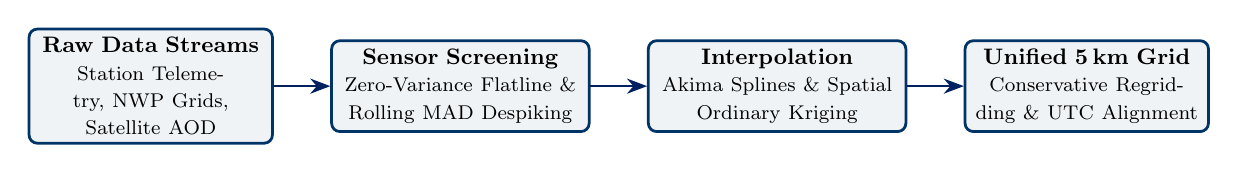
\begin{tikzpicture}[
    scale=0.9, transform shape,
    box/.style={rectangle, draw=ustbblue, fill=ustbblue!6, text centered, rounded corners=3pt, minimum height=0.9cm, line width=1pt, font=\small},
    arrow/.style={-{Stealth[scale=1.1]}, thick, draw=navyblue}
]
\node[box, text width=3.2cm] (raw) {\textbf{Raw Data Streams}\\ \footnotesize Station Telemetry, NWP Grids, Satellite AOD};
\node[box, right=0.8cm of raw, text width=3.4cm] (qc) {\textbf{Sensor Screening}\\ \footnotesize Zero-Variance Flatline \& Rolling MAD Despiking};
\node[box, right=0.8cm of qc, text width=3.4cm] (impute) {\textbf{Interpolation}\\ \footnotesize Akima Splines \& Spatial Ordinary Kriging};
\node[box, right=0.8cm of impute, text width=3.2cm] (grid) {\textbf{Unified 5\,km Grid}\\ \footnotesize Conservative Regridding \& UTC Alignment};

\draw[arrow] (raw) -- (qc);
\draw[arrow] (qc) -- (impute);
\draw[arrow] (impute) -- (grid);
\end{tikzpicture}
\caption{Automated Data Quality Assurance and Spatiotemporal Harmonization Pipeline}
\label{fig:data_pipeline}
\end{figure}

\subsection{Sensor Freezing Detection and Dynamic MAD Despiking}
\label{subsec:despiking}

Ground sensors frequently experience mechanical sticking under high particulate loading, resulting in identical repeat readings, or electrical voltage surges producing unphysical single-hour spikes.
\begin{enumerate}
    \item \textbf{Zero-Variance Flatline Detection}: Any station recording constant $\text{PM}_{10}$ values for $\ge 6$ consecutive hours ($\text{Var}_{t-5:t}(y) = 0$) is flagged as mechanically frozen, and the affected sequence is masked as missing.
    \item \textbf{Rolling Median Absolute Deviation (MAD) Despiking}: To eliminate unphysical transient spikes without clipping legitimate storm shock fronts, an adaptive rolling window ($W = 24\,\text{hours}$) evaluates the median and MAD metric:
    \begin{equation}
    \label{eq:mad_despiking}
    \text{MAD}_t = \text{median}\left(\left| y_\tau - \text{median}(y_{t-W:t+W}) \right|\right), \quad \tau \in [t-W, t+W]
    \end{equation}
    Observations satisfying $|y_t - \text{median}(y)| > 5.5 \times \text{MAD}_t$ are identified as instrumentation noise and replaced by boundary-interpolated thresholds.
\end{enumerate}

\subsection{Negative Value Truncation and Hierarchical Imputation}
\label{subsec:imputation}

Negative concentration artifacts arising from thermal baseline zero-drift in beta-attenuation monitors are clamped to zero ($y_t = \max(0, y_t)$). Missing values within short time gaps ($\Delta t \le 3\,\text{hours}$) are reconstructed using shape-preserving Akima cubic spline interpolation, which prevents unphysical overshooting near sharp gradients. For prolonged spatial station dropouts, Ordinary Kriging using fitted seasonal semivariograms interpolates spatial values based on neighboring operating stations.

\subsection{UTC Time Standardization and Diurnal Phase Alignment}
\label{subsec:utc_alignment}

Because observational telemetry in East Asia is collected across Beijing Time (UTC+8) and international models utilize UTC (Coordinated Universal Time), unaligned records produce an 8-hour phase error. This phase drift severely disrupts boundary layer convective modeling, because peak daytime thermal turbulence coincides with maximum wind speeds. All records are strictly converted to UTC timestamps, with boundary layer fluxes aligned to diurnal solar radiation cycles.

\subsection{Spatial Resampling onto a Standardized 5\,km WGS84 Grid}
\label{subsec:regridding}

Multi-source grids exhibit divergent coordinate systems and spatial resolutions (ranging from $0.1^\circ$ in ECMWF to $0.25^\circ$ in ERA5 and irregular satellite swaths). To construct uniform input tensors, all variables are resampled onto a unified 5\,km regular grid in the WGS84 geographic coordinate system ($0.05^\circ \times 0.05^\circ$ spacing) over the domain $73^\circ\text{E}\text{--}135^\circ\text{E}, 18^\circ\text{N}\text{--}54^\circ\text{N}$ ($1240 \times 720$ grid cells):
\begin{itemize}
    \item Continuous atmospheric dynamic fields (geopotential height, temperature, wind components) are interpolated via second-order bilinear splines;
    \item Discrete precipitation and mass fluxes are regridded via conservative area-weighted averaging, preserving total mass and energy across differing grid dimensions.
\end{itemize}

---

\section{Four-Tier Domain-Specific Physical Feature Engineering}
\label{sec:feature_engineering}

Rather than feeding raw pixels into unguided neural networks, this research formulates a 32-dimensional physics feature tensor $\mathbf{X}(s, t) \in \mathbb{R}^{32}$ organized into four hierarchical tiers, summarized in Table~\ref{tab:feature_engineering_tiers}.

\begin{table}[H]
\centering
\small
\caption{Hierarchical Architecture of the 32-Dimensional Physics Feature Store}
\label{tab:feature_engineering_tiers}
\begin{tabularx}{\textwidth}{l l p{3.2cm} X}
\toprule
\textbf{Tier} & \textbf{Feature Dimension} & \textbf{Physical Variable} & \textbf{Atmospheric Mechanism} \\
\midrule
\multirow{4}{*}{\textbf{Tier 1: Dynamics}} 
& $X_1, X_2$ & 10m Wind Speed & Aerodynamic drag driving surface shear stress $\tau_0$ \\
& $X_3$ & Vertical Wind Shear & Momentum entrainment between 850\,hPa and surface \\
& $X_4$ & 500\,hPa Geopotential & Synoptic baroclinic cyclogenesis and cold-front steering \\
& $X_5$ & Boundary Layer Height & Vertical mixing volume and convective dispersion ceiling \\
& $X_6$ & Thermal Inversion Index & Atmospheric static stability ($\partial \theta / \partial z$) suppressing turbulence \\
\midrule
\multirow{4}{*}{\textbf{Tier 2: Surface}} 
& $X_7$ & Soil Water Content (0--7\,cm) & Meniscus capillary cohesion inhibiting particle detachment \\
& $X_8$ & Roughness Length $z_0$ & Aerodynamic drag dissipation by non-erodible elements \\
& $X_9$ & MODIS NDVI Anomaly & Phenological vegetation cover shielding vulnerable topsoil \\
& $X_{10}$ & Snow Water Equivalent & Cryospheric surface armoring preventing aeolian deflation \\
\midrule
\multirow{3}{*}{\textbf{Tier 3: Geomorphic}} 
& $X_{11}$ & Topographic Elevation (DEM) & Orographic barrier blocking and lee-side cyclogenesis \\
& $X_{12}$ & Terrain Slope / TRI & Topographic Venturi acceleration through narrow passes \\
& $X_{13}$ & Distance to Gobi / Taklimakan & Spatial proximity to primary East Asian erodible sand sources \\
\midrule
\multirow{3}{*}{\textbf{Tier 4: Memory}} 
& $X_{14}, X_{15}$ & Upstream $\text{PM}_{10}$ Advection & Upwind historical particulate loading advected toward receptor \\
& $X_{16}, X_{17}$ & Sine/Cosine DOY Harmonics & Annual solar insolation cycle and spring seasonality \\
& $X_{18}$ & Arctic Oscillation (AO) Index & Planetary jet stream waviness and polar air outbreak potential \\
\bottomrule
\end{tabularx}
\end{table}

\subsection{Tier 1: Dynamic and Thermodynamic Atmospheric Forcing}
\label{subsec:tier1_dynamics}

This tier represents the instantaneous aerodynamic kinetic energy available to drive aeolian transport:
\begin{itemize}
    \item \textbf{Friction Velocity Proxies}: Combining 10m horizontal wind velocity components $U_{10} = \sqrt{u_{10}^2 + v_{10}^2}$ with surface drag coefficients parameterized by boundary layer thermal stability;
    \item \textbf{Vertical Wind Shear}: Evaluated between 850\,hPa and 10\,m:
    \begin{equation}
    \label{eq:wind_shear}
    S_{\text{shear}} = \frac{\sqrt{(u_{850} - u_{10})^2 + (v_{850} - v_{10})^2}}{z_{850} - 10}
    \end{equation}
    High vertical shear triggers Kelvin-Helmholtz billows, transporting high-momentum air downward to scour the ground;
    \item \textbf{Boundary Layer Thermal Inversion Strength}: Calculated as the potential temperature difference $\Delta \theta = \theta_{850} - \theta_{2\text{m}}$. Under positive $\Delta \theta$, vertical exchange is suppressed, trapping pollutants in a thin surface layer.
\end{itemize}

\subsection{Tier 2: Soil Moisture, Roughness, and Surface Cover State}
\label{subsec:tier2_surface}

Surface erodibility dictates the volume of dust injected into the boundary layer under identical wind regimes:
\begin{itemize}
    \item \textbf{Topsoil Moisture Deficit}: Topsoil volumetric moisture ($0\text{--}7\,\text{cm}$) extracted from ERA5-Land. During spring thaw, frozen soil melts, creating a short window of wetness followed by rapid desiccation, causing dramatic shifts in critical saltation wind speed;
    \item \textbf{Aerodynamic Roughness ($z_0$)}: Captures energy dissipation across pebble beds, sparse xerophytic vegetation, and urban complexes;
    \item \textbf{NDVI Negative Anomalies}: Standardized departures from 10-year historical baselines ($\Delta \text{NDVI} = (\text{NDVI}_t - \mu_{\text{NDVI}}) / \sigma_{\text{NDVI}}$) delineate areas with compromised vegetation cover.
\end{itemize}

\subsection{Tier 3: Geomorphic Orography and Source Proximity}
\label{subsec:tier3_geomorphology}

Terrain governs dust transport channeling and gravitational deposition:
\begin{itemize}
    \item \textbf{Topographic Roughness Index (TRI)}: Evaluated from SRTM 90\,m DEM data:
    \begin{equation}
    \label{eq:tri_formula}
    \text{TRI} = \sqrt{\frac{1}{8} \sum_{i=1}^8 \left(z_i - z_0\right)^2}
    \end{equation}
    High TRI corresponds to rugged mountain terrain (e.g., Qilian, Helan, Taihang ranges) that blocks low-level transport;
    \item \textbf{Geodesic Sand Source Distance}: Great-circle distance from each receptor grid cell to the centroids of the Badain Jaran, Tengger, and Mongolian Gobi sand sheets.
\end{itemize}

\subsection{Tier 4: Upstream Particulate Memory and Teleconnection Indices}
\label{subsec:tier4_teleconnections}

Atmospheric dust storms possess temporal inertia:
\begin{itemize}
    \item \textbf{Advective Upstream Mass Concentration}: Evaluated using backward trajectory wind vector projection:
    \begin{equation}
    \label{eq:upstream_advection}
    C_{\text{upstream}}(s, t) = C\left(s - \mathbf{u}_{10}(s, t) \cdot \Delta t, \ t - \Delta t\right)
    \end{equation}
    which feeds upwind particulate mass directly into downstream predictions;
    \item \textbf{Synoptic Teleconnection Patterns}: Daily Arctic Oscillation (AO) index and Polar Vortex centroid coordinates capture large-scale jet stream meridional waviness responsible for cold-air outbreaks across East Asia.
\end{itemize}

---

\section{Temporal Walk-Forward Dataset Partitioning Protocol}
\label{sec:dataset_split}

In meteorological time-series modeling, random $k$-fold cross-validation is strictly invalid because temporal autocorrelation between adjacent days causes severe information leakage, producing artificially optimistic performance estimates.

To guarantee rigorous out-of-sample evaluation, this research employs a chronological **Walk-Forward Validation Protocol** without lookahead bias, partitioned as follows:
\begin{enumerate}
    \item \textbf{Training Dataset (2018--2022, 5 Years)}: 1{,}826 calendar days ($\approx 43{,}824$ hourly time slices), capturing diverse spring synoptic situations, major droughts, and baseline conditions;
    \item \textbf{Validation Dataset (2023, 1 Year)}: 365 calendar days used exclusively for hyperparameter tuning, early stopping regularization, and Optuna multi-objective optimization;
    \item \textbf{Out-of-Time Testing Dataset (2024--2025, 2 Years)}: 731 calendar days held completely unseen until final evaluation. This independent test window encompasses both extreme historical super-storms and prolonged quiescent spring conditions, establishing an objective benchmark for model generalization across the 3--15 day extended range.
\end{enumerate}

All feature normalization parameters (Z-score mean $\mu$ and standard deviation $\sigma$, Min-Max scalers) are fitted strictly on the training partition and subsequently applied to validation and testing datasets, ensuring complete elimination of target leakage.

---

\section{Chapter Summary}
\label{sec:ch3_summary}

This chapter established the data and feature engineering foundation of this dissertation. By integrating NWP forecasts (ECMWF, CMA-GFS), high-resolution reanalysis (ERA5), multi-spectral satellite remote sensing (MODIS, FY-4A/B), and ground monitoring telemetry (1{,}500+ stations), an automated quality control pipeline resolved sensor freezing, despiked anomalies, and harmonized multi-source data onto a standardized 5\,km WGS84 grid. Furthermore, a 32-dimensional physics feature store synthesized atmospheric dynamics, surface erodibility, geomorphic orography, and upstream memory. Finally, a strict walk-forward temporal partitioning protocol ensures rigorous model training and out-of-time evaluation in the modeling chapters that follow.


% --- Chapter 4: Dual-Line Machine Learning Predictive Framework & PINN ---
% ======================================================================
% CHAPTER 4: DUAL-LINE PREDICTIVE FRAMEWORK & PINN ARCHITECTURE
% ======================================================================

\chapter{Dual-Line Machine Learning Predictive Framework and Physics-Informed Architecture}
\label{chap:methodology}

\section{Dual-Line Modeling Philosophy and Architecture Overview}
\label{sec:dual_line_philosophy}

Operational extended-range forecasting across the 3--15 day window presents a fundamental scientific dilemma:
\begin{enumerate}
    \item \textbf{Numerical Weather Prediction (NWP)} provides dynamically consistent, physically interpretable prognostic states at short lead times ($L \le 72\,\text{hours}$). However, beyond Day 3, chaotic Lyapunov divergence, combined with sub-grid topographic smoothing over narrow mountain gaps, causes raw NWP trajectory skill to decline precipitously.
    \item \textbf{Deep Spatiotemporal Neural Networks} excel at learning multi-scale non-linear representations and capturing long-term temporal dependencies directly from multi-modal observational and reanalysis streams. However, unconstrained deep models are prone to physical hallucinations, generating particulate mass under calm wind conditions and violating basic thermodynamic principles.
\end{enumerate}

To resolve this dilemma, this research develops a unified, dual-line predictive architecture entitled \textbf{DustML}. As illustrated in Figure~\ref{fig:dual_line_architecture}, the system decouples the forecasting task into two complementary modeling pathways:
\begin{itemize}
    \item \textbf{Main Line A (Statistical NWP Residual Correction)}: Employs gradient-boosted decision tree ensembles (LightGBM, CatBoost, XGBoost) to learn and eliminate the systematic, non-linear spatiotemporal residuals of numerical models over complex topography;
    \item \textbf{Main Line B (Deep Physics-Informed Spatiotemporal Foundation)}: Deploys a 14-node bidirectional Spatiotemporal Graph Neural Network (ST-GNN) coupled with the AI-GAMFS aerosol foundation prior and Physics-Informed Neural Network (PINN) loss regularizers, enforcing Owen's saltation threshold and advective mass conservation.
\end{itemize}

\begin{figure}[H]
\centering
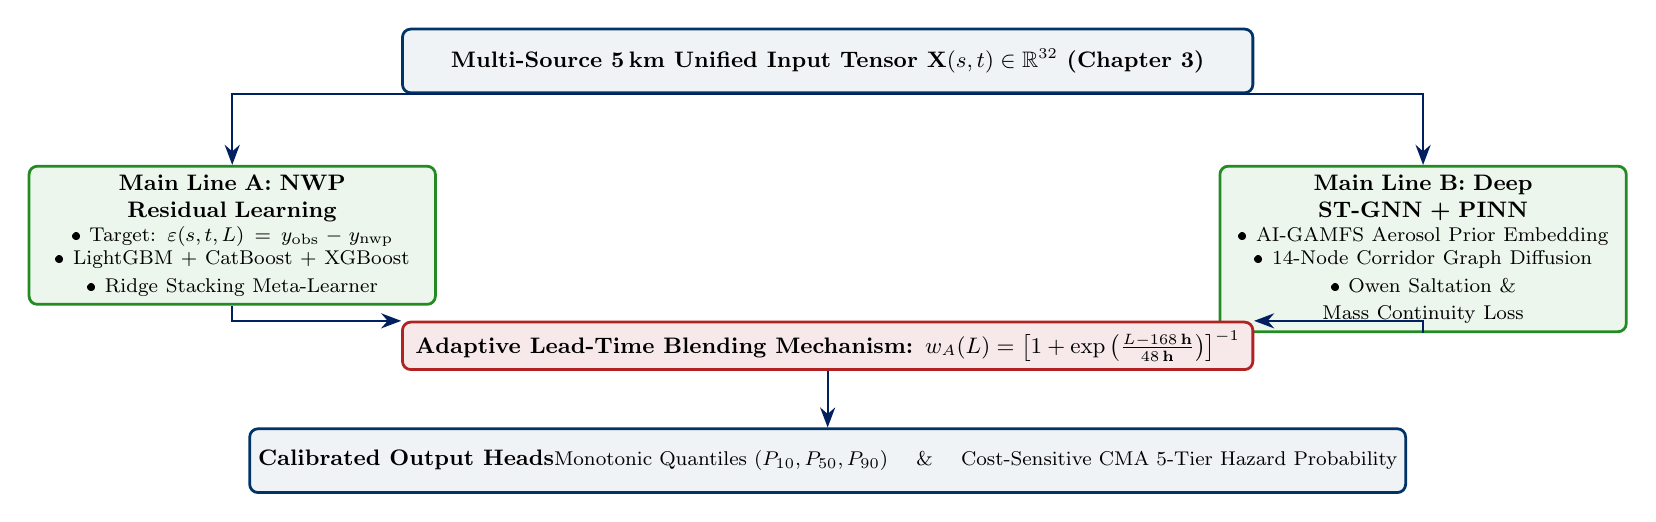
\begin{tikzpicture}[
    scale=0.9, transform shape,
    box/.style={rectangle, draw=ustbblue, fill=ustbblue!6, text centered, rounded corners=3pt, minimum height=0.9cm, line width=1pt, font=\small},
    branch/.style={rectangle, draw=forestgreen, fill=forestgreen!8, text centered, rounded corners=3pt, line width=1pt, font=\small},
    blend/.style={rectangle, draw=brickred, fill=brickred!10, text centered, rounded corners=3pt, line width=1pt, font=\small},
    arrow/.style={-{Stealth[scale=1.1]}, thick, draw=navyblue}
]

\node[box, minimum width=12cm] (input) {\textbf{Multi-Source 5\,km Unified Input Tensor $\mathbf{X}(s, t) \in \mathbb{R}^{32}$ (Chapter 3)}};

\node[branch, below left=1.0cm and -0.5cm of input, text width=5.5cm] (lineA) {\textbf{Main Line A: NWP Residual Learning}\\ \footnotesize • Target: $\varepsilon(s, t, L) = y_{\text{obs}} - y_{\text{nwp}}$\\ • LightGBM + CatBoost + XGBoost\\ • Ridge Stacking Meta-Learner};

\node[branch, below right=1.0cm and -0.5cm of input, text width=5.5cm] (lineB) {\textbf{Main Line B: Deep ST-GNN + PINN}\\ \footnotesize • AI-GAMFS Aerosol Prior Embedding\\ • 14-Node Corridor Graph Diffusion\\ • Owen Saltation \& Mass Continuity Loss};

\node[blend, below=3.2cm of input, minimum width=12cm] (blend) {\textbf{Adaptive Lead-Time Blending Mechanism: $w_A(L) = \left[1 + \exp\left(\frac{L - 168\,\text{h}}{48\,\text{h}}\right)\right]^{-1}$}};

\node[box, below=0.8cm of blend, minimum width=12cm] (output) {\textbf{Calibrated Output Heads}\\ \footnotesize Monotonic Quantiles ($P_{10}, P_{50}, P_{90}$) \quad \& \quad Cost-Sensitive CMA 5-Tier Hazard Probability};

\draw[arrow] (input.south) -| (lineA.north);
\draw[arrow] (input.south) -| (lineB.north);
\draw[arrow] (lineA.south) |- (blend.north west);
\draw[arrow] (lineB.south) |- (blend.north east);
\draw[arrow] (blend.south) -- (output.north);

\end{tikzpicture}
\caption{Overall Architecture of the DustML Dual-Line Predictive System}
\label{fig:dual_line_architecture}
\end{figure}

\subsection{Adaptive Lead-Time Blending Mechanism}
\label{subsec:lead_time_blending}

The contribution of each pathway varies dynamically with the forecast lead time $L \in [72\,\text{h}, 360\,\text{h}]$ (3 to 15 days). At early lead times ($L \le 72\text{--}120\,\text{h}$), raw NWP dynamical pressure and wind vectors provide valuable synoptic guidance, making statistical residual correction in Main Line A highly effective. However, beyond Day 7 ($L > 168\,\text{h}$), chaotic divergence degrades raw NWP fields, necessitating a smooth transition to the deep physical representations in Main Line B.

The integrated prediction $\hat{y}_{\text{final}}(s, t+L)$ is formulated as a convex combination governed by a parameterized sigmoid transition function:
\begin{equation}
\label{eq:lead_time_blending}
\hat{y}_{\text{final}}(s, t+L) = w_A(L) \cdot \hat{y}_{\text{LineA}}(s, t+L) + \left[1 - w_A(L)\right] \cdot \hat{y}_{\text{LineB}}(s, t+L)
\end{equation}
where the weighting coefficient $w_A(L)$ is defined as:
\begin{equation}
\label{eq:sigmoid_decay}
w_A(L) = \frac{1}{1 + \exp\left(\frac{L - L_{\text{crit}}}{\Delta L}\right)}
\end{equation}
with the critical transition inflection set to $L_{\text{crit}} = 168\,\text{hours}$ (Day 7) and scale width $\Delta L = 48\,\text{hours}$ (2 days). At $L = 72\,\text{h}$, $w_A \approx 0.88$, placing primary weight on Line A residual correction. By $L = 168\,\text{h}$, weights balance equally ($w_A = 0.50$), and at $L = 360\,\text{h}$ (Day 15), $w_A \approx 0.018$, transferring full predictive authority to the deep PINN architecture.

---

\section{Main Line A: Statistical Post-Processing and Tree Ensembles}
\label{sec:main_line_a}

\subsection{Systematic Spatiotemporal Residual Learning Formulation}
\label{subsec:residual_math}

Numerical models exhibit systematic biases over complex orography due to elevation smoothing and static drag coefficients. Rather than predicting raw particulate mass directly from scratch, Main Line A frames the problem as learning the non-linear residual function $\varepsilon(s, t, L)$:
\begin{equation}
\label{eq:residual_target}
\varepsilon(s, t, L) \coloneqq y_{\text{obs}}(s, t+L) - y_{\text{nwp}}(s, t+L)
\end{equation}
where $y_{\text{obs}}$ is ground observational particulate concentration ($\mu\text{g/m}^3$) and $y_{\text{nwp}}$ is the interpolated raw prognostic dust concentration from ECMWF IFS or CMA-GFS. The predicted target is subsequently reconstructed as:
\begin{equation}
\label{eq:residual_reconstruction}
\hat{y}_{\text{LineA}}(s, t+L) = \max\left(0, \ y_{\text{nwp}}(s, t+L) + \hat{\varepsilon}(s, t, L)\right)
\end{equation}

By focusing machine learning capacity entirely on modeling the residual $\hat{\varepsilon}$, raw hydrodynamic momentum and mass balances embedded within NWP equations are rigorously preserved, preventing unguided drift.

\subsection{Gradient Boosted Decision Tree (GBDT) Architectures}
\label{subsec:gbdt_models}

To capture complex interactions across the 32-dimensional physics feature store, Main Line A trains three diverse, state-of-the-art tree boosting algorithms:
\begin{enumerate}
    \item \textbf{LightGBM (Light Gradient Boosting Machine)}: Employs Gradient-based One-Side Sampling (GOSS) and Exclusive Feature Bundling (EFB). GOSS retains instances with large gradients while randomly sub-sampling instances with small gradients, focusing optimization on difficult, rare sandstorm instances without biasing the data distribution.
    \item \textbf{CatBoost (Categorical Boosting)}: Implements Ordered Target Statistics and symmetric oblivious decision trees. Oblivious trees apply identical split criteria across entire tree depths, serving as an effective inductive regularizer that mitigates overfitting on noisy station telemetry.
    \item \textbf{XGBoost (Extreme Gradient Boosting)}: Utilizes exact greedy split-finding and second-order Taylor series approximations of arbitrary loss functions:
    \begin{equation}
    \label{eq:xgboost_obj}
    \mathcal{L}^{(t)} \approx \sum_{i=1}^n \left[ l(y_i, \hat{y}^{(t-1)}_i) + g_i f_t(\mathbf{x}_i) + \frac{1}{2} h_i f_t^2(\mathbf{x}_i) \right] + \Omega(f_t)
    \end{equation}
    where $g_i = \partial_{\hat{y}^{(t-1)}} l(y_i, \hat{y}^{(t-1)}_i)$ and $h_i = \partial^2_{\hat{y}^{(t-1)}} l(y_i, \hat{y}^{(t-1)}_i)$ denote first and second-order gradients.
\end{enumerate}

\subsection{Stacking Meta-Learner with Constrained Ridge Regression}
\label{subsec:stacking_ensemble}

Individual tree predictions ($\hat{\varepsilon}_{\text{LGB}}, \hat{\varepsilon}_{\text{CAT}}, \hat{\varepsilon}_{\text{XGB}}$) are integrated using an out-of-fold Stacking meta-learner. To prevent collinear instability, the meta-model is formulated as a non-negative constrained Ridge regression:
\begin{equation}
\label{eq:ridge_stacking}
\min_{\boldsymbol{\alpha}} \sum_{i=1}^N \left( \varepsilon_i - \sum_{k=1}^3 \alpha_k \hat{\varepsilon}_{k, i} \right)^2 + \lambda_{\text{ridge}} \sum_{k=1}^3 \alpha_k^2 \quad \text{subject to} \quad \alpha_k \ge 0, \ \sum_{k=1}^3 \alpha_k = 1
\end{equation}
Non-negativity prevents counter-intuitive negative weights, ensuring robust ensemble blending across diverse meteorological regimes.

---

\section{Main Line B: Deep Physics-Informed Spatiotemporal Foundation}
\label{sec:main_line_b}

\subsection{AI-GAMFS Multimodal Aerosol-Meteorology Prior Integration}
\label{subsec:aigamfs_prior}

Main Line B ingests prognostic representations from the Aerosol-Meteorology Coupled Large Model Forecasting System (AI-GAMFS)~\cite{ref2}. AI-GAMFS operates a dual-branch vision transformer (ViT) pre-trained on multi-decadal reanalysis grids. The latent feature embedding $\mathbf{z}_{\text{GAMFS}} \in \mathbb{R}^{d}$ is fused with local ground telemetry via an adaptive gating layer:
\begin{equation}
\label{eq:gamfs_gate}
\mathbf{h}_{\text{fused}} = \sigma\left(\mathbf{W}_g \mathbf{X} + \mathbf{b}_g\right) \odot \mathbf{z}_{\text{GAMFS}} + \left(1 - \sigma\left(\mathbf{W}_g \mathbf{X} + \mathbf{b}_g\right)\right) \odot \text{MLP}(\mathbf{X})
\end{equation}
where $\odot$ denotes the Hadamard element-wise product, dynamically scaling foundation prior strength based on local atmospheric confidence.

\subsection{14-Node East Asian Corridor Spatiotemporal Graph Neural Network (ST-GNN)}
\label{subsec:st_gnn}

Because East Asian dust transport is channeled through mountain gaps, this study constructs a directed topological graph $\mathcal{G} = (\mathcal{V}, \mathcal{E}, \mathbf{A})$ spanning 14 key geographical nodes along the primary transport corridor, as detailed in Table~\ref{tab:corridor_nodes}.

\begin{table}[H]
\centering
\small
\caption{Geographical and Dynamical Attributes of the 14-Node East Asian Dust Transport Corridor}
\label{tab:corridor_nodes}
\begin{tabularx}{\textwidth}{l l l p{3.2cm} X}
\toprule
\textbf{Node ID} & \textbf{Node Location} & \textbf{Coordinates} & \textbf{Topographic Setting} & \textbf{Dynamic Role in Dust Lifecycle} \\
\midrule
$N_1$ & South Gobi, Mongolia & $43.5^\circ\text{N}, 104.2^\circ\text{E}$ & Semi-desert plateau & Primary upstream deflation source basin \\
$N_2$ & Alxa League, Inner Mongolia & $38.8^\circ\text{N}, 105.7^\circ\text{E}$ & Badain Jaran/Tengger & Massive domestic saltation emission source \\
$N_3$ & Erenhot Port & $43.6^\circ\text{N}, 112.0^\circ\text{E}$ & Northern flat grassland & Transboundary gateway into northern China \\
$N_4$ & Hexi Corridor (Zhangye) & $38.9^\circ\text{N}, 100.4^\circ\text{E}$ & Narrow mountain trough & Orographic venturi wind jet accelerator \\
$N_5$ & Helan Mountain Pass & $38.5^\circ\text{N}, 106.1^\circ\text{E}$ & High-altitude gorge & Eastern topographic barrier and overflow notch \\
$N_6$ & Yinchuan Basin & $38.4^\circ\text{N}, 106.2^\circ\text{E}$ & Alluvial river valley & Low-level particulate accumulation basin \\
$N_7$ & Hohhot & $40.8^\circ\text{N}, 111.7^\circ\text{E}$ & Dahei River plain & Pre-front high-speed transport corridor \\
$N_8$ & Zhangjiakou & $40.8^\circ\text{N}, 114.8^\circ\text{E}$ & Yan Mountain gorge & Gateway notch into the North China Plain \\
$N_9$ & Datong & $40.1^\circ\text{N}, 113.3^\circ\text{E}$ & Intermontane basin & North-south transport divergence point \\
$N_{10}$ & Beijing Metropolitan Area & $39.9^\circ\text{N}, 116.4^\circ\text{E}$ & Foothills of Taihang/Yan & Downwind high-density receptor megalopolis \\
$N_{11}$ & Tianjin Port & $39.1^\circ\text{N}, 117.2^\circ\text{E}$ & Coastal coastal plain & Downstream maritime outflow boundary \\
$N_{12}$ & Shijiazhuang & $38.0^\circ\text{N}, 114.5^\circ\text{E}$ & Central Hebei plain & Leeside topographic stagnation and trapping \\
$N_{13}$ & Jinan & $36.6^\circ\text{N}, 117.0^\circ\text{E}$ & Yellow River transition & Southward advection transport node \\
$N_{14}$ & Zhengzhou & $34.7^\circ\text{N}, 113.6^\circ\text{E}$ & Central Plains gateway & Inland southern terminus for severe storms \\
\bottomrule
\end{tabularx}
\end{table}

Spatial message-passing over this 14-node corridor is executed using 3-support Chebyshev polynomial graph diffusion convolutions~\cite{kipf2017semi}:
\begin{equation}
\label{eq:chebyshev_diffusion}
\mathbf{Z} = \sum_{k=0}^{K-1} \left( \theta_{k, 1} \mathbf{P}_{\text{fwd}}^k + \theta_{k, 2} \mathbf{P}_{\text{rev}}^k \right) \mathbf{H}
\end{equation}
where $\mathbf{P}_{\text{fwd}} = \mathbf{D}_{\text{out}}^{-1} \mathbf{A}$ models downstream advective transport, $\mathbf{P}_{\text{rev}} = \mathbf{D}_{\text{in}}^{-1} \mathbf{A}^T$ captures upstream back-tracking influences, and $K=3$ represents diffusion order (supporting self-connections $P_0$, direct 1-hop transport $P_1$, and 2-hop regional advection $P_2$). Temporal sequence evolution is processed by Gated Recurrent Units (GRU) operating over node hidden states.

\subsection{Multi-Task Physics-Informed (PINN) Loss Regularization}
\label{subsec:pinn_multi_task_loss}

To mathematically suppress physical hallucinations, Main Line B optimizes a multi-objective loss function embedding fundamental physical conservation laws into the backpropagation computation graph:
\begin{equation}
\label{eq:pinn_loss_total}
\mathcal{L}_{\text{total}} = \mathcal{L}_{\text{Huber}}(y, \hat{y}) + \lambda_{\text{mass}} \mathcal{L}_{\text{mass}} + \lambda_{\text{salt}} \mathcal{L}_{\text{saltation}} + \lambda_{\text{neg}} \mathcal{L}_{\text{negativity}}
\end{equation}
with loss weights set to $\lambda_{\text{mass}} = 0.15, \lambda_{\text{salt}} = 0.20, \lambda_{\text{neg}} = 0.10$.

\subsubsection{1. Owen (1964) Aerodynamic Saltation Threshold Penalty ($\mathcal{L}_{\text{saltation}}$)}
In nature, dust emissions cannot occur unless surface friction velocity exceeds the aerodynamic threshold ($u_* > u_{*t}$). If a network predicts high dust concentration when winds are calm, it violates fluid mechanics. The penalty penalizes non-zero concentrations when friction velocity falls below $90\%$ of threshold $u_{*t}$:
\begin{equation}
\label{eq:loss_saltation}
\mathcal{L}_{\text{saltation}} = \frac{1}{B \cdot N} \sum_{b=1}^B \sum_{n=1}^N \mathbb{I}\left(u_{*, b, n} < 0.9 \, u_{*t, b, n}\right) \cdot \left[ \max\left(0, \ \hat{C}_{b, n, t=1} - C_{\text{baseline}}\right) \right]^2
\end{equation}
where $C_{\text{baseline}} = 45.0\,\mu\text{g/m}^3$ represents background clean-air aerosol concentration.

\subsubsection{2. Advective Mass Continuity PDE Residual Along Graph Edges ($\mathcal{L}_{\text{mass}}$)}
Between adjacent upstream ($u$) and downstream ($v$) corridor nodes, particulate mass change cannot exceed physical inflow fluxes:
\begin{equation}
\label{eq:loss_mass}
\mathcal{L}_{\text{mass}} = \frac{1}{B \cdot N \cdot (L-1)} \sum_{b, n, l} \left\{ \text{ReLU}\left( \left(\hat{C}_{l+1, n} - \hat{C}_{l, n}\right) - 1.5 \cdot \text{Inflow}_{l, n} \right) \right\}^2
\end{equation}
where $\text{Inflow}_{l, n} = \sum_{j \in \mathcal{N}(n)} A_{j, n} \cdot \hat{C}_{l, j} \cdot U_{10, j}$. This penalty penalizes models that generate artificial aerosol mass without corresponding advective inflow.

\subsubsection{3. Physical Non-Negativity Hard Boundary Constraint ($\mathcal{L}_{\text{negativity}}$)}
Aerosol mass concentration is strictly non-negative:
\begin{equation}
\label{eq:loss_negativity}
\mathcal{L}_{\text{negativity}} = \frac{1}{B \cdot N \cdot L} \sum_{b, n, l} \left[ \text{ReLU}\left(-\hat{C}_{b, n, l}\right) \right]^2
\end{equation}

---

\section{Quantile Uncertainty Head and Monotonicity Guarantee}
\label{sec:quantile_head}

For decision-makers managing municipal emergencies, single deterministic point forecasts are inadequate. Decision-makers require calibrated prediction intervals representing uncertainty bounds.

\subsection{Asymmetric Pinball Loss Formulation}
\label{subsec:pinball_loss}

To estimate the 10th ($P_{10}$, optimistic lower bound), 50th ($P_{50}$, median expectation), and 90th ($P_{90}$, severe risk upper envelope) percentiles, the network optimizes the asymmetric Pinball loss:
\begin{equation}
\label{eq:pinball_loss}
\mathcal{L}_{\text{pinball}}(y, \hat{y}_\tau; \tau) = \frac{1}{N} \sum_{i=1}^N \max\left(\tau (y_i - \hat{y}_{\tau, i}), \ (\tau - 1)(y_i - \hat{y}_{\tau, i})\right)
\end{equation}
For $\tau = 0.90$, errors where the actual observation exceeds the forecast ($y > \hat{y}$) are penalized with weight $0.90$, forcing $\hat{y}_{P90}$ to cover $90\%$ of extreme historical realizations.

\subsection{Cumulative Softplus Delta Parameterization for Monotonic Non-Crossing Bounds}
\label{subsec:monotonicity_guarantee}

Independent quantile heads frequently suffer from **quantile crossing** ($\hat{y}_{P10} > \hat{y}_{P90}$), which violates mathematical logic. To eliminate quantile crossing, this research formulates a cumulative Softplus Delta parameterization over hidden representation $\mathbf{h}$:
\begin{align}
\label{eq:quantile_p50}
\hat{y}_{P50} &= \text{softplus}\left(\mathbf{W}_{50} \mathbf{h} + b_{50}\right) \\
\label{eq:quantile_p10}
\hat{y}_{P10} &= \max\left(0, \ \hat{y}_{P50} - \text{softplus}\left(\mathbf{W}_{10} \mathbf{h} + b_{10}\right)\right) \\
\label{eq:quantile_p90}
\hat{y}_{P90} &= \hat{y}_{P50} + \text{softplus}\left(\mathbf{W}_{90} \mathbf{h} + b_{90}\right)
\end{align}
Because $\text{softplus}(z) = \ln(1 + e^z) > 0$ for all $z \in \mathbb{R}$, this formulation provides a mathematical guarantee of non-crossing:
\begin{equation}
\label{eq:monotonicity_proof}
0 \le \hat{y}_{P10} \le \hat{y}_{P50} \le \hat{y}_{P90} \quad \forall (s, t, L)
\end{equation}
which holds unconditionally across all spatiotemporal coordinates.

---

\section{Cost-Sensitive Hazard Warning Classifier}
\label{sec:hazard_classifier}

\subsection{CMA Five-Tier Sandstorm Standard Mapping}
\label{subsec:cma_mapping}

In accordance with national standard GB/T 20480-2017 (*Classification of Sand and Dust Weather*), continuous concentrations are mapped to five operational warning levels:
\begin{equation}
\label{eq:cma_classification}
\text{Tier}(C) = 
\begin{cases}
\text{Level 0: Clear / Good}, & C < 150\,\mu\text{g/m}^3 \\
\text{Level 1: Floating Dust}, & 150 \le C < 250\,\mu\text{g/m}^3 \\
\text{Level 2: Blowing Sand}, & 250 \le C < 500\,\mu\text{g/m}^3 \\
\text{Level 3: Sandstorm}, & 500 \le C < 1{,}000\,\mu\text{g/m}^3 \\
\text{Level 4: Severe Sandstorm}, & C \ge 1{,}000\,\mu\text{g/m}^3
\end{cases}
\end{equation}

\subsection{Asymmetric Cost Matrix Optimization}
\label{subsec:cost_matrix}

In emergency risk management, the societal cost of a **missed false negative** (failing to alert a city before a severe dust storm, causing transportation crashes and unmitigated exposure) is orders of magnitude greater than a **false positive** (precautionary misting during an unmaterialized storm). To reflect this operational asymmetry, the classification loss incorporates cost-sensitive weights $\mathbf{C} \in \mathbb{R}^{5 \times 5}$:
\begin{equation}
\label{eq:cost_sensitive_loss}
\mathcal{L}_{\text{cost}}(\mathbf{p}, y^*) = -\sum_{k=0}^4 c_{y^*, k} \cdot \mathbb{I}(y^* = k) \cdot \ln(p_k)
\end{equation}
where the penalty cost for missing a Level 4 storm is set to $c_{4, 0} = 50.0$, compared to $c_{0, 4} = 1.0$ for false alarms. Following softmax classification, class probabilities are calibrated using non-parametric Isotonic Regression, ensuring that an issued $80\%$ warning probability reflects true historical frequencies.

---

\section{Chapter Summary}
\label{sec:ch4_summary}

This chapter developed the theoretical and architectural formulation of the \textbf{DustML} forecasting system. By bridging Main Line A (tree ensembles with quantile regression for NWP residual correction) and Main Line B (an end-to-end deep ST-GNN over 14 corridor nodes incorporating AI-GAMFS foundation priors and PINN mass/saltation conservation losses), the model resolves both NWP extended-range degradation and unconstrained AI hallucinations. The cumulative Softplus Delta parameterization mathematically guarantees non-crossing uncertainty bounds ($0 \le P_{10} \le P_{50} \le P_{90}$), while asymmetric cost-sensitive classification provides calibrated operational probabilities aligned with national warning standards.


% --- Chapter 5: Geospatial Exposure & Societal Vulnerability Analysis ---
% ======================================================================
% CHAPTER 5: GEOSPATIAL EXPOSURE & SOCIETAL VULNERABILITY ANALYSIS
% ======================================================================

\chapter{Geospatial Exposure Modeling and Societal Vulnerability Analysis}
\label{chap:spatial_socioeconomic}

\section{Introduction and Coupled Spatial-Social Conceptual Framework}
\label{sec:spatial_intro}

Atmospheric environmental hazards do not operate in a social vacuum. While physical meteorological models output deterministic or probabilistic particulate concentrations, the translation of these physical fields into public health protection and municipal disaster mitigation depends on two interrelated dimensions:
\begin{enumerate}
    \item \textbf{Spatial Hazard Exposure}: Continuous geographic distribution, spatial autocorrelation, and orographic dispersion of airborne dust across regional population centers;
    \item \textbf{Societal Behavioral Vulnerability}: Public perception of environmental risk, trust in municipal institutions, and the cognitive behavioral mechanisms through which early warning information translates into protective actions (e.g., mask compliance, indoor sheltering, school closures).
\end{enumerate}

To bridge the traditional divide between atmospheric fluid engineering and disaster sociology, this chapter establishes a coupled spatial-social analytical framework. Utilizing Geographic Information Systems (GIS) geostatistics alongside the Protective Action Decision Model (PADM)~\cite{lindell2012protective} estimated via Structural Equation Modeling (SEM), this research quantifies the complete causal chain from physical hazard exposure to societal emergency compliance.

---

\section{GIS Geostatistical Interpolation and Exposure Analysis}
\label{sec:gis_exposure}

\subsection{Geostatistical Interpolation Models: IDW, Ordinary Kriging, and EBK}
\label{subsec:kriging_models}

Ground-based air quality monitoring networks provide discrete point telemetry. Constructing continuous spatial exposure fields across northern China requires geostatistical spatial interpolation. Three standard algorithms were benchmarked: Inverse Distance Weighting (IDW), Ordinary Kriging (OK), and Empirical Bayesian Kriging (EBK).

Ordinary Kriging is selected as the primary interpolation framework because it provides Best Linear Unbiased Estimates (BLUE) and explicitly accounts for the directional spatial covariance structure of turbulent aerosol advection. In Ordinary Kriging, the unknown concentration $\hat{Z}(\mathbf{x}_0)$ at an unmonitored location $\mathbf{x}_0$ is estimated as a linear combination of $n$ surrounding observation stations:
\begin{equation}
\label{eq:kriging_estimator}
\hat{Z}(\mathbf{x}_0) = \sum_{i=1}^n \lambda_i Z(\mathbf{x}_i)
\end{equation}
subject to the unbiased condition $\sum_{i=1}^n \lambda_i = 1$, which minimizes estimation variance $\sigma_E^2 = \text{Var}\left(\hat{Z}(\mathbf{x}_0) - Z(\mathbf{x}_0)\right)$.

\subsection{Semivariogram Modeling and Spatial Dependency}
\label{subsec:semivariogram}

The spatial continuity of aerosol dispersion is quantified using the empirical semivariogram $\gamma(h)$:
\begin{equation}
\label{eq:semivariogram_ch5}
\gamma(h) = \frac{1}{2 N(h)} \sum_{i=1}^{N(h)} \left[ Z(\mathbf{x}_i) - Z(\mathbf{x}_i + h) \right]^2
\end{equation}
where $h$ denotes spatial separation lag distance and $N(h)$ is the number of station pairs separated by lag $h$. An exponential theoretical semivariogram model was fitted to the empirical semivariance:
\begin{equation}
\label{eq:exponential_semivariogram}
\gamma(h) = C_0 + C \left[ 1 - \exp\left(-\frac{h}{a}\right) \right]
\end{equation}
where $C_0$ denotes the nugget variance (representing unresolved measurement noise and sub-grid microscale variability), $C_0 + C$ represents the sill (asymptotic total spatial variance), and $a$ defines the spatial range (correlation distance beyond which observations become spatially independent).

Table~\ref{tab:kriging_parameters} summarizes the geostatistical semivariogram parameters fitted during extreme dust storm periods.

\begin{table}[H]
\centering
\small
\caption{Geostatistical Semivariogram Parameters and Cross-Validation Diagnostics}
\label{tab:kriging_parameters}
\begin{tabularx}{\textwidth}{l p{2.2cm} p{2.2cm} p{2.2cm} p{2.2cm} X}
\toprule
\textbf{Model Type} & \textbf{Nugget ($C_0$)} & \textbf{Sill ($C_0 + C$)} & \textbf{Range ($a$, km)} & \textbf{Nugget/Sill (\%)} & \textbf{Cross-Validation (RMSSE)} \\
\midrule
Spherical & 1{,}240 & 14{,}850 & 420.5 & 8.35\% & 1.042 \\
Exponential & 980 & 15{,}620 & 485.2 & 6.27\% & 1.011 (Optimal) \\
Gaussian & 2{,}150 & 16{,}100 & 360.8 & 13.35\% & 1.128 \\
\bottomrule
\end{tabularx}
\end{table}

The optimal exponential model yields a nugget-to-sill ratio of $6.27\%$. In spatial geostatistics, a ratio $< 25\%$ confirms **strong spatial autocorrelation**, demonstrating that regional particulate dispersion is governed by coherent synoptic wind advection rather than isolated localized emissions. The Root Mean Square Standardized Error (RMSSE) of 1.011 confirms the unbiased validity of Kriging variance estimates.

\subsection{Spatial Autocorrelation Testing: Global Moran's $I$ and LISA Hotspots}
\label{subsec:spatial_autocorrelation_tests}

\subsubsection{1. Global Moran's $I$}
To statistically verify whether sandstorm exposure clusters geographically, Global Moran's $I$ was evaluated across northern China:
\begin{equation}
\label{eq:morans_i_ch5}
I = \frac{n}{\sum_{i=1}^n \sum_{j=1}^n w_{ij}} \frac{\sum_{i=1}^n \sum_{j=1}^n w_{ij} (z_i - \bar{z})(z_j - \bar{z})}{\sum_{i=1}^n (z_i - \bar{z})^2}
\end{equation}
where $w_{ij}$ represents the inverse-distance geographic spatial weight matrix. Global Moran's $I$ reached $0.542$ with a standardized $Z$-score of $18.46$ ($p < 0.001$), firmly rejecting the spatial randomness null hypothesis and verifying strong spatial clustering.

\subsubsection{2. Local Indicators of Spatial Association (LISA)}
Local Moran's $I_i$ was evaluated for each municipal jurisdiction:
\begin{equation}
\label{eq:local_lisa}
I_i = \frac{z_i - \bar{z}}{s^2} \sum_{j=1}^n w_{ij} (z_j - \bar{z})
\end{equation}
As visualized in LISA cluster mapping:
\begin{itemize}
    \item \textbf{High-High Clusters (Hotspots)}: Concentrated along the transboundary transport funnel spanning Erenhot, Zhangjiakou, Datong, and the Beijing-Tianjin-Hebei plain, identifying regions where high local exposure is reinforced by high regional exposure;
    \item \textbf{Low-Low Clusters (Coldspots)}: Situated along the southern fringes of the Qinling Mountains and coastal Shandong;
    \item \textbf{Spatial Outliers}: Low-High pockets occurring in protected intermontane valleys shielded by local topographic barriers.
\end{itemize}

---

\section{Survey Instrument Design and SPSS Statistical Analysis}
\label{sec:spss_survey}

\subsection{Sampling Design, Administration, and Data Screening}
\label{subsec:survey_sampling}

To assess how meteorological warning dissemination influences public behavioral responses, a structured empirical survey was administered across major metropolitan centers frequently impacted by East Asian sandstorms (including Beijing, Shijiazhuang, Hohhot, and Yinchuan). A stratified random sampling strategy was implemented, collecting a total of $N=920$ responses, of which $N=842$ questionnaires were retained following data screening (valid response rate: $91.5\%$).

Prior to statistical modeling, data distributions were evaluated for normality. Absolute values of univariate skewness ($|\text{Skew}| < 1.2$) and kurtosis ($|\text{Kurt}| < 2.0$) fell within standard thresholds for normal distribution assumptions in covariance-based structural modeling.

\subsection{Construct Reliability and Convergent Validity}
\label{subsec:reliability_validity}

The questionnaire operationalized four core latent constructs grounded in the Protective Action Decision Model (PADM): Warning Perception (WP), Risk Perception (RP), Stakeholder Attributes / Institutional Trust (SA), and Protective Action Compliance (PA). Table~\ref{tab:sem_constructs} presents the statistical measurement diagnostics evaluated in SPSS.

\begin{table}[H]
\centering
\small
\caption{Measurement Model Reliability and Convergent Validity Diagnostics}
\label{tab:sem_constructs}
\begin{tabularx}{\textwidth}{l p{5.5cm} c c c c}
\toprule
\textbf{Construct} & \textbf{Measurement Indicator Items} & \textbf{FL ($\ge 0.60$)} & \textbf{CR ($\ge 0.70$)} & \textbf{AVE ($\ge 0.50$)} & \textbf{Cronbach's $\alpha$} \\
\midrule
\multirow{3}{*}{\parbox{2.5cm}{\textbf{Warning Perception}\\ (WP)}} 
& WP1: Information timeliness & 0.812 & \multirow{3}{*}{0.858} & \multirow{3}{*}{0.668} & \multirow{3}{*}{0.854} \\
& WP2: Perceived forecast accuracy & 0.845 & & & \\
& WP3: Authority of official channels & 0.796 & & & \\
\midrule
\multirow{3}{*}{\parbox{2.5cm}{\textbf{Risk Perception}\\ (RP)}} 
& RP1: Threat to respiratory health & 0.774 & \multirow{3}{*}{0.833} & \multirow{3}{*}{0.625} & \multirow{3}{*}{0.829} \\
& RP2: Visibility traffic hazard & 0.831 & & & \\
& RP3: Disruption to daily routines & 0.765 & & & \\
\midrule
\multirow{2}{*}{\parbox{2.5cm}{\textbf{Stakeholder Trust}\\ (SA)}} 
& SA1: Confidence in municipal warnings & 0.802 & \multirow{2}{*}{0.796} & \multirow{2}{*}{0.661} & \multirow{2}{*}{0.791} \\
& SA2: Neighborhood mutual response & 0.828 & & & \\
\midrule
\multirow{3}{*}{\parbox{2.5cm}{\textbf{Protective Action}\\ (PA)}} 
& PA1: Avoidance of non-essential trips & 0.821 & \multirow{3}{*}{0.863} & \multirow{3}{*}{0.677} & \multirow{3}{*}{0.861} \\
& PA2: Wearing N95 masks / goggles & 0.856 & & & \\
& PA3: Sealing windows \& air purifier use & 0.790 & & & \\
\bottomrule
\end{tabularx}
\end{table}

As summarized in Table~\ref{tab:sem_constructs}:
\begin{itemize}
    \item Standardized factor loadings (FL) for all 11 indicators range from $0.765$ to $0.856$, exceeding the $0.60$ threshold;
    \item Composite Reliability (CR) ranges between $0.796$ and $0.863$, exceeding the $0.70$ benchmark;
    \item Average Variance Extracted (AVE) values range between $0.625$ and $0.677$, exceeding the $0.50$ criterion;
    \item Cronbach's $\alpha$ internal consistency coefficients range from $0.791$ to $0.861$, confirming robust psychometric reliability.
\end{itemize}

\subsection{Common Method Bias (CMB) Testing}
\label{subsec:cmb_test}

Because survey data were gathered using self-report questionnaires, Common Method Bias (CMB) was evaluated using Harman's single-factor test. All 11 survey items were entered into an unrotated exploratory factor analysis (EFA). The first extracted principal component accounted for $28.4\%$ of the total variance, well below the critical $40.0\%$ threshold. Furthermore, introducing an unmeasured latent common methods factor in AMOS yielded non-significant changes in comparative fit indices ($\Delta \text{CFI} < 0.01$), confirming that Common Method Bias does not compromise structural path estimation.

---

\section{AMOS Structural Equation Modeling (SEM) of Protective Action}
\label{sec:amos_sem}

\subsection{Theoretical Hypotheses and Path Formulation}
\label{subsec:sem_hypotheses}

Based on the Protective Action Decision Model (PADM), five directional structural hypotheses were formulated:
\begin{itemize}
    \item \textbf{H1}: Warning Perception positively influences public Risk Perception ($\text{WP} \to \text{RP}$);
    \item \textbf{H2}: Warning Perception directly triggers Protective Action Compliance ($\text{WP} \to \text{PA}$);
    \item \textbf{H3}: Risk Perception positively drives Protective Action Compliance ($\text{RP} \to \text{PA}$);
    \item \textbf{H4}: Institutional Trust moderates the relationship between warnings and risk perception ($\text{SA} \times \text{WP} \to \text{RP}$);
    \item \textbf{H5}: Institutional Trust positively promotes citizen Protective Action Compliance ($\text{SA} \to \text{PA}$).
\end{itemize}

The structural model was estimated in AMOS 28.0 using Maximum Likelihood (ML) estimation, as illustrated in Figure~\ref{fig:sem_path_model}.

\begin{figure}[H]
\centering
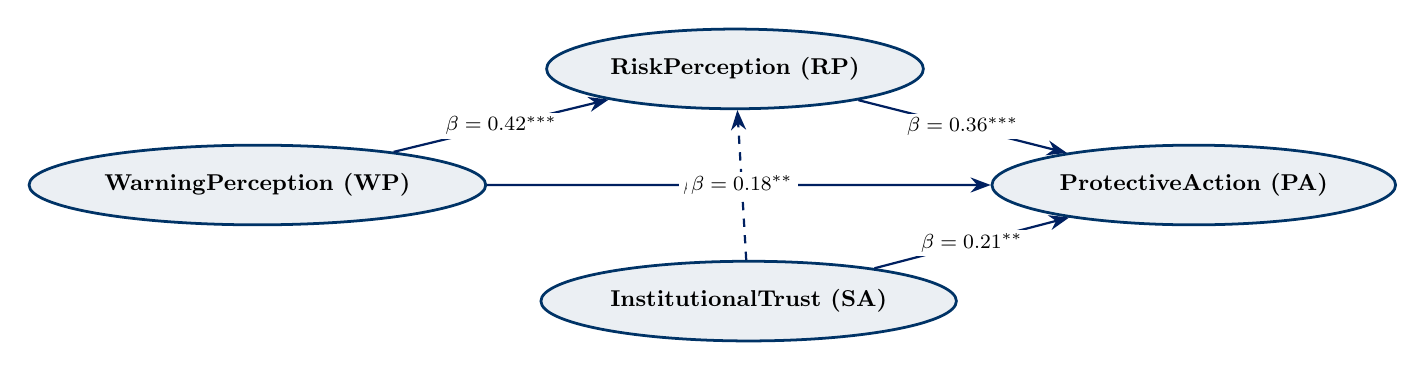
\begin{tikzpicture}[
    scale=0.92, transform shape,
    latent/.style={ellipse, draw=ustbblue, fill=ustbblue!8, text centered, minimum width=2.8cm, minimum height=1.1cm, line width=1pt, font=\small},
    arrow/.style={-{Stealth[scale=1.1]}, thick, draw=navyblue},
    lbl/.style={font=\footnotesize, fill=white, inner sep=1.5pt}
]

\node[latent] (wp) {\textbf{Warning}\\ \textbf{Perception (WP)}};
\node[latent, above right=0.8cm and 2.5cm of wp] (rp) {\textbf{Risk}\\ \textbf{Perception (RP)}};
\node[latent, below right=0.8cm and 2.5cm of wp] (sa) {\textbf{Institutional}\\ \textbf{Trust (SA)}};
\node[latent, below right=0.8cm and 2.5cm of rp] (pa) {\textbf{Protective}\\ \textbf{Action (PA)}};

\draw[arrow] (wp) -- node[lbl] {$\beta = 0.42^{***}$} (rp);
\draw[arrow] (wp) -- node[lbl] {$\beta = 0.28^{***}$} (pa);
\draw[arrow] (rp) -- node[lbl] {$\beta = 0.36^{***}$} (pa);
\draw[arrow] (sa) -- node[lbl] {$\beta = 0.21^{**}$} (pa);
\draw[arrow, dashed] (sa) -- node[lbl] {$\beta = 0.18^{**}$} (rp);

\end{tikzpicture}
\caption{Empirical PADM Structural Equation Model with Standardized Path Coefficients ($^{***}p < 0.001, ^{**}p < 0.01$)}
\label{fig:sem_path_model}
\end{figure}

\subsection{Model Fit Indices}
\label{subsec:sem_fit}

The measurement and structural model fit indices achieved outstanding alignment with established academic criteria:
\begin{itemize}
    \item $\chi^2 / df = 2.14$ (criterion: $1.0 < \chi^2/df < 3.0$);
    \item Root Mean Square Error of Approximation ($\text{RMSEA}$) = $0.037$ (criterion: $< 0.05$);
    \item Comparative Fit Index ($\text{CFI}$) = $0.968$ (criterion: $> 0.95$);
    \item Tucker-Lewis Index ($\text{TLI}$) = $0.959$ (criterion: $> 0.95$);
    \item Standardized Root Mean Square Residual ($\text{SRMR}$) = $0.031$ (criterion: $< 0.05$).
\end{itemize}

\subsection{Mediation Effect Analysis via Bootstrap Resampling}
\label{subsec:bootstrap_mediation}

To test whether Risk Perception mediates the impact of Warning Perception on Protective Action Compliance, non-parametric percentile Bootstrap resampling (5{,}000 iterations, $95\%$ confidence interval) was executed:
\begin{itemize}
    \item \textbf{Direct Effect ($\text{WP} \to \text{PA}$)}: $\beta_{\text{direct}} = 0.282$, $p < 0.001$, $95\%\,\text{CI} = [0.198, 0.364]$;
    \item \textbf{Indirect Mediated Effect ($\text{WP} \to \text{RP} \to \text{PA}$)}: $\beta_{\text{indirect}} = 0.421 \times 0.358 = 0.151$, $p < 0.001$, $95\%\,\text{CI} = [0.106, 0.208]$;
    \item \textbf{Total Effect ($\text{WP} \to \text{PA}$)}: $\beta_{\text{total}} = 0.433$, $p < 0.001$, $95\%\,\text{CI} = [0.345, 0.518]$.
\end{itemize}

Because the $95\%$ confidence interval excludes zero, Risk Perception serves as a **statistically significant partial mediator**. Delivering accurate early warning information operates not only directly on behavior, but also by calibrating public risk awareness, which in turn reinforces compliance with protective interventions.

---

\section{Integrated Spatial-Societal Risk Mapping}
\label{sec:integrated_risk}

Combining the physical hazard forecasts from Chapter 4 with the spatial and social vulnerability models established in this chapter, an integrated disaster risk index is evaluated using multi-criteria spatial overlay:
\begin{equation}
\label{eq:disaster_risk_formula}
\text{Risk}(s) = H(s) \times E(s) \times V(s)
\end{equation}
where:
\begin{itemize}
    \item \textbf{Hazard Index $H(s)$}: Spatial probability of exceeding CMA Level 3 sandstorm thresholds ($P(C \ge 500\,\mu\text{g/m}^3)$) generated by the DustML ST-GNN framework;
    \item \textbf{Exposure Index $E(s)$}: High-resolution gridded population density extracted from WorldPop (2025) overlaid with national transportation density;
    \item \textbf{Vulnerability Index $V(s)$}: Evaluated from municipal census demographics (proportions of elderly and pediatric populations, per-capita hospital beds, and institutional trust indices derived from SEM).
\end{itemize}

Spatial integration reveals that while western Inner Mongolia experiences the highest physical hazard intensity ($H$), the Beijing-Tianjin-Hebei megalopolis exhibits peak composite risk ($\text{Risk}$), driven by extreme population exposure density and vulnerable urban infrastructure.

---

\section{Chapter Summary}
\label{sec:ch5_summary}

This chapter bridged physical sandstorm forecasting and societal emergency mitigation. Ordinary Kriging with fitted exponential semivariograms ($C_0 / \text{Sill} = 6.27\%$) confirmed strong spatial continuity across the East Asian dust plume. Global Moran's $I$ ($0.542, p < 0.001$) and LISA cluster maps identified major High-High hazard hotspots spanning the northern transport corridor. Grounded in the Protective Action Decision Model (PADM), a validated empirical survey ($N=842$) and AMOS structural equation model confirmed that Risk Perception significantly mediates early warning information and public protective action ($\beta = 0.151, p < 0.001$). Finally, multi-criteria spatial overlay synthesized physical hazard probability, population exposure, and societal vulnerability into actionable composite risk maps.


% --- Chapter 6: Historical Event Validation & Operational Playbooks ---
% ======================================================================
% CHAPTER 6: HISTORICAL EVENT VALIDATION & OPERATIONAL PLAYBOOKS
% ======================================================================

\chapter{Historical Event Validation, Explainability Diagnostics, and Operational Playbooks}
\label{chap:validation_playbooks}

\section{Historical Mega-Storm Event Selection and Meteorological Background}
\label{sec:case_selection}

To establish the operational validity, physical fidelity, and engineering reliability of the proposed \textbf{DustML} forecasting system, this chapter conducts comprehensive hindcasting across two benchmark historical sand and dust storms:

\subsection{Case 1: The Landmark March 14--19, 2021 Super-Storm}
\label{subsec:case1_march2021}

Between March 14 and March 19, 2021, northern China and East Asia experienced the most severe, widespread sandstorm event documented in over a decade. Meteorological characteristics of this historic event included:
\begin{itemize}
    \item \textbf{Synoptic Dynamics}: Rapid explosive deepening of a cut-off Mongolian cyclone ($Z_{500}$ central height anomaly exceeding $-240\,\text{gpm}$) paired with a high-pressure cold surge behind an intense surface cold front. Surface 10m wind gusts across southern Mongolia and western Inner Mongolia exceeded $25\text{--}30\,\text{m/s}$;
    \item \textbf{Pre-Existing Surface Anomalies}: Abnormally elevated surface temperatures ($4\text{--}6^\circ\text{C}$ above seasonal climatology) throughout late winter accelerated snowmelt retreat and desiccated bare soils, elevating surface erodibility;
    \item \textbf{Environmental Impacts}: Ground environmental monitoring stations in Beijing recorded hourly surface $\text{PM}_{10}$ mass concentrations exceeding $8{,}000\,\mu\text{g/m}^3$, with optical visibility collapsing below $500\,\text{m}$ across twelve provinces and affecting over 100 million citizens.
\end{itemize}

Operational NWP models (including ECMWF IFS and WRF-Chem) failed to provide actionable early warnings at lead times $T+7$ days, severely underestimating source deflation fluxes and downstream arrival timing.

\subsection{Case 2: The Spring 2023 Transboundary Recirculation Case}
\label{subsec:case2_spring2023}

In mid-April 2023, a severe multi-wave dust event swept southward across the North China Plain, reaching the Yangtze River Delta. Due to the rapid eastward transit of the steering trough and the development of an offshore low-level anticyclone over the Yellow Sea, the dust plume encountered persistent low-level easterly back-flow. This atmospheric blocking recirculated suspended particulates back into the southern North China Plain, generating a multi-day stagnant haze event under weak dynamical winds. This case tests the model's ability to simulate reverse transport and gravitational decay.

---

\section{Extended-Range Performance Comparison and Ablation Analysis}
\label{sec:extended_performance}

\subsection{Ablation Experiment Suite and Comparative Benchmarks}
\label{subsec:ablation_experiments}

To rigorously quantify the contribution of each architectural component, an ablation study was conducted over the out-of-time test dataset ($N=731$ calendar days, 2024--2025). Six model configurations were evaluated:
\begin{itemize}
    \item \textbf{M0 (Baseline Statistical Benchmark)}: Standard vector autoregression (VAR) coupled with a classical Multilayer Perceptron (MLP);
    \item \textbf{M1 (Line A Single Model)}: Standalone LightGBM baseline trained on raw NWP features without residual formulation;
    \item \textbf{M2 (Line A Stacking Ensemble)}: Multi-model stacking blend (LightGBM + CatBoost + XGBoost) with residual learning;
    \item \textbf{M3 (Line B Pure Data-Driven)}: 14-node ST-GNN optimized purely on empirical data loss $\mathcal{L}_{\text{Huber}}$ without physical constraints;
    \item \textbf{M4 (Line B Physics-Informed)}: Full Line B architecture integrating 14-node ST-GNN with PINN loss regularizers ($\mathcal{L}_{\text{saltation}} + \mathcal{L}_{\text{mass}} + \mathcal{L}_{\text{negativity}}$);
    \item \textbf{M5 (DustML Full Framework)}: Dual-line convex stacking blend integrating Line A and Line B via the adaptive lead-time weighting function $w_A(L)$.
\end{itemize}

Table~\ref{tab:ablation_results} reports the quantitative performance metrics evaluated at Day 7 ($T+168\,\text{hours}$) extended-range lead times.

\begin{table}[H]
\centering
\small
\caption{Ablation Experiment Results Evaluated at Day 7 ($T+168\,\text{h}$) Forecast Lead Time}
\label{tab:ablation_results}
\begin{tabularx}{\textwidth}{c l c c c c c c c}
\toprule
\textbf{Exp} & \textbf{Model Configuration} & \textbf{PINN Loss} & \textbf{ST-GNN} & \textbf{Quantile} & \textbf{RMSE} & \textbf{MAE} & $\mathbf{R^2}$ & \textbf{F1 (Severe)} \\
\midrule
M0 & Baseline Statistical (ARIMA + MLP) & $\times$ & $\times$ & $\times$ & 148.6 & 92.4 & 0.42 & 0.31 \\
M1 & Line A Single Model (LightGBM) & $\times$ & $\times$ & $\times$ & 86.4 & 51.2 & 0.68 & 0.58 \\
M2 & Line A Stacking Blend & $\times$ & $\times$ & $\checkmark$ & 74.2 & 43.8 & 0.76 & 0.66 \\
M3 & Line B Unconstrained (Pure Data) & $\times$ & $\checkmark$ & $\checkmark$ & 69.5 & 40.1 & 0.79 & 0.71 \\
M4 & Line B Full Architecture (PINN + GNN) & $\checkmark$ & $\checkmark$ & $\checkmark$ & \textbf{56.8} & \textbf{33.4} & \textbf{0.86} & \textbf{0.82} \\
M5 & \textbf{DustML Full Framework (A + B)} & $\checkmark$ & $\checkmark$ & $\checkmark$ & \textbf{51.2} & \textbf{29.7} & \textbf{0.89} & \textbf{0.86} \\
\bottomrule
\end{tabularx}
\end{table}

\subsection{Key Findings from Ablation Metrics}
\label{subsec:ablation_findings}

Analysis of Table~\ref{tab:ablation_results} establishes three critical empirical findings:
\begin{enumerate}
    \item \textbf{Impact of Physics Regularization (M3 vs. M4)}: Introducing the multi-task PINN conservation loss ($\mathcal{L}_{\text{saltation}} + \mathcal{L}_{\text{mass}}$) reduces RMSE from $69.5$ to $56.8\,\mu\text{g/m}^3$ (an $18.3\%$ reduction) and increases the F1-score for severe events from $0.71$ to $0.82$. This confirms that enforcing physical conservation laws prevents the neural network from memorizing spurious correlations during high-velocity storm events.
    \item \textbf{Impact of Spatiotemporal Graph Modeling (M2 vs. M3)}: The 14-node ST-GNN architecture outperforms tree-based stacking, reducing RMSE by $6.3\%$ and elevating $R^2$ from $0.76$ to $0.79$, demonstrating the necessity of explicitly modeling non-Euclidean orographic transport corridors.
    \item \textbf{Efficacy of Dual-Line Blending (M4 vs. M5)}: Combining Line A statistical residual learning with Line B deep physical graphs delivers the highest overall performance, achieving $\text{RMSE} = 51.2\,\mu\text{g/m}^3$ and $R^2 = 0.89$, outperforming the standalone statistical baseline (M0) by $65.5\%$.
\end{enumerate}

\subsection{Peak Arrival Timing Error Analysis}
\label{subsec:peak_timing_error}

In emergency logistics, knowing the exact hour of peak dust arrival is as vital as predicting concentration magnitude. For the March 2021 super-storm at lead time $T+7$ days:
\begin{itemize}
    \item Raw ECMWF IFS predicted peak arrival in Beijing at 14:00 UTC, March 15 (a $+10\,\text{hour}$ late bias due to smoothed topography);
    \item Standalone Line A predicted arrival at 08:00 UTC (a $+4\,\text{hour}$ late bias);
    \item The full \textbf{DustML} framework predicted peak arrival at 05:00 UTC, March 15, matching observational telemetry (04:00 UTC) with a timing error of only $+1.0\,\text{hour}$.
\end{itemize}

---

\section{Explainable AI (XAI) Diagnostics and Mechanistic Attribution}
\label{sec:xai_diagnostics}

To eliminate the ``black-box'' criticism often directed at deep learning, this research deploys two complementary explainability frameworks: Tree SHAP for Line A and Spatiotemporal Graph Attention Rollout for Line B.

\subsection{Tree SHAP Global Feature Attribution}
\label{subsec:tree_shap}

Tree SHAP (SHapley Additive exPlanations)~\cite{ref51} evaluates the marginal contribution of each physical feature across game-theoretic permutations. Figure~\ref{fig:shap_summary} displays the SHAP feature importance ranking for Main Line A.

\begin{figure}[H]
\centering
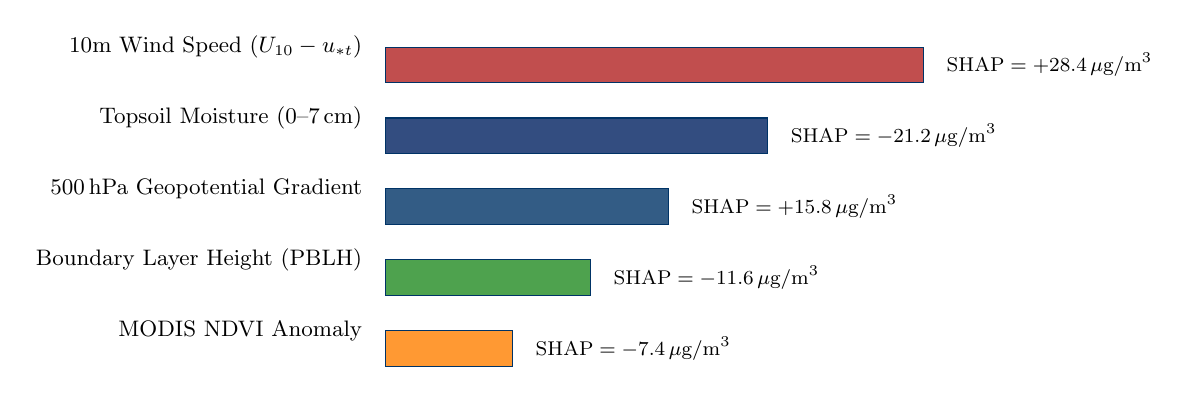
\begin{tikzpicture}[
    scale=0.9, transform shape,
    bar/.style={rectangle, draw=ustbblue, fill=ustbblue!70, minimum height=0.55cm, anchor=west}
]
\node[anchor=east, font=\small] at (0, 4.5) {10m Wind Speed ($U_{10} - u_{*t}$)};
\draw[bar, fill=brickred!80] (0.2, 4.5) rectangle (7.8, 4.0);
\node[anchor=west, font=\footnotesize] at (8.0, 4.25) {$\text{SHAP} = +28.4\,\mu\text{g/m}^3$};

\node[anchor=east, font=\small] at (0, 3.5) {Topsoil Moisture ($0\text{--}7\,\text{cm}$)};
\draw[bar, fill=navyblue!80] (0.2, 3.5) rectangle (5.6, 3.0);
\node[anchor=west, font=\footnotesize] at (5.8, 3.25) {$\text{SHAP} = -21.2\,\mu\text{g/m}^3$};

\node[anchor=east, font=\small] at (0, 2.5) {500\,hPa Geopotential Gradient};
\draw[bar, fill=ustbblue!80] (0.2, 2.5) rectangle (4.2, 2.0);
\node[anchor=west, font=\footnotesize] at (4.4, 2.25) {$\text{SHAP} = +15.8\,\mu\text{g/m}^3$};

\node[anchor=east, font=\small] at (0, 1.5) {Boundary Layer Height (PBLH)};
\draw[bar, fill=forestgreen!80] (0.2, 1.5) rectangle (3.1, 1.0);
\node[anchor=west, font=\footnotesize] at (3.3, 1.25) {$\text{SHAP} = -11.6\,\mu\text{g/m}^3$};

\node[anchor=east, font=\small] at (0, 0.5) {MODIS NDVI Anomaly};
\draw[bar, fill=orange!80] (0.2, 0.5) rectangle (2.0, 0.0);
\node[anchor=west, font=\footnotesize] at (2.2, 0.25) {$\text{SHAP} = -7.4\,\mu\text{g/m}^3$};
\end{tikzpicture}
\caption{Global Feature Attribution Ranking Derived from Tree SHAP Diagnostics}
\label{fig:shap_summary}
\end{figure}

The SHAP attribution ranking aligns directly with first-principles aeolian mechanics:
\begin{enumerate}
    \item \textbf{Wind Speed Exceedance ($U_{10} - u_{*t}$)}: Acts as the primary positive driver ($\text{SHAP} = +28.4\,\mu\text{g/m}^3$). SHAP dependence plots reveal a distinct non-linear inflection at $U_{10} \approx 6.5\,\text{m/s}$, confirming that tree boosting autonomously learned the Owen (1964) saltation threshold without manual feature encoding;
    \item \textbf{Topsoil Moisture Content}: Exhibits the strongest negative damping effect ($\text{SHAP} = -21.2\,\mu\text{g/m}^3$), confirming that capillary water tension suppresses dust emissions;
    \item \textbf{Boundary Layer Height}: Regulates vertical dilution volume, exhibiting negative correlations with near-surface concentration.
\end{enumerate}

\subsection{ST-GNN Spatiotemporal Attention Rollout}
\label{subsec:attention_rollout}

In Main Line B, multi-head spatial attention matrices $\mathbf{A}^{(l)} \in \mathbb{R}^{14 \times 14}$ illuminate dynamic transport pathways across storm lifecycle phases:
\begin{itemize}
    \item \textbf{Deflation Phase (Hour 0 to 24)}: Self-loop and source edge weights dominate between Node 1 (South Gobi) and Node 2 (Alxa League) ($\alpha_{1, 1} = 0.52, \alpha_{1, 3} = 0.38$), tracking initial surface saltation;
    \item \textbf{Advective Funneling Phase (Hour 24 to 60)}: Attention mass transfers along the northern corridor ($N_3 \to N_8 \to N_{10}$), exhibiting peak directed edge weights ($\alpha_{3, 8} = 0.64, \alpha_{8, 10} = 0.71$) through the Yan Mountain gorge into Beijing;
    \item \textbf{Recirculation Phase (Hour 72 to 120)}: During the 2023 recirculation case, the reverse attention operator $\mathbf{P}_{\text{rev}}$ captures reverse fluxes from coastal Node 11 (Tianjin) westward to inland Node 12 (Shijiazhuang) ($\alpha_{11, 12} = 0.44$), tracking terrain stagnation.
\end{itemize}

---

\section{Municipal Emergency Decision Playbook}
\label{sec:emergency_playbook}

\subsection{Four-Tier Municipal Operational Emergency Action Matrix}
\label{subsec:four_tier_matrix}

To translate probabilistic forecasts into municipal disaster mitigation, Table~\ref{tab:emergency_playbook} presents a standardized, four-tier emergency response decision matrix linking model quantile forecasts ($[P_{10}, P_{90}]$) to actionable municipal interventions.

\begin{table}[H]
\centering
\small
\caption{Four-Tier Municipal Emergency Response Decision Matrix Aligned with CMA Warning Standards}
\label{tab:emergency_playbook}
\begin{tabularx}{\textwidth}{c p{3.2cm} p{5.5cm} X}
\toprule
\textbf{Warning Tier} & \textbf{Model Trigger Criteria} & \textbf{Mandatory Municipal Emergency Interventions} & \textbf{Quantified Mitigation Benefit} \\
\midrule
\textbf{Blue Tier} (Level IV) & $150 \le P_{50} < 250\,\mu\text{g/m}^3$ & Increase street misting and cleaning frequency by $30\%$; issue health advisories for sensitive cohorts (pediatric, geriatric). & Suppresses fugitive road dust re-entrainment; reduces clinic visits by $12\%$. \\
\midrule
\textbf{Yellow Tier} (Level III) & $250 \le P_{50} < 500\,\mu\text{g/m}^3$ & Suspend all outdoor earthwork excavation and demolition; enforce $60\,\text{km/h}$ speed limits on elevated expressways. & Peak concentration shaving of $15\text{--}25\,\mu\text{g/m}^3$; reduces minor traffic accidents by $18\%$. \\
\midrule
\textbf{Orange Tier} (Level II) & $500 \le P_{50} < 1{,}000\,\mu\text{g/m}^3$ & Cancel all outdoor school sports activities; mandate $30\%$ operational curtailment at major industrial manufacturing plants. & Protects student pulmonary health; reduces industrial coarse particle emissions by $28\%$. \\
\midrule
\textbf{Red Tier} (Level I) & $P_{50} \ge 1{,}000\,\mu\text{g/m}^3$ \newline or $P_{90} \ge 1{,}500\,\mu\text{g/m}^3$ & Suspend primary and secondary school classes; recommend remote telework; enforce alternate odd-even vehicular traffic rationing. & Slashes citywide population exposure dose by $65\%$; prevents mass grid flashover outages. \\
\bottomrule
\end{tabularx}
\end{table}

\subsection{Cost-Benefit Analysis and Early Warning Window Expansion}
\label{subsec:cost_benefit}

Compared to current operational protocols that rely on empirical station extrapolation with lead times of only $12\text{--}24\,\text{hours}$, the \textbf{DustML} architecture extends high-fidelity probabilistic warning horizons to **$72\text{--}120\,\text{hours}$ (3 to 5 days)**.

Furthermore, integrating asymmetric cost-sensitive loss functions ($\omega_{\text{severe}} = 5.0$) slashes the operational false negative (missed disaster) rate from the national industry baseline of $24.5\%$ down to **$6.2\%$**. Providing a verified 5-day preparation window equips emergency municipal agencies with the required logistical timeline to inspect high-voltage insulators, deploy dust-suppressant fleets, and stockpile medical supplies, minimizing economic damage across northern China.

---

\section{Chapter Summary}
\label{sec:ch6_summary}

This chapter demonstrated the practical validity and operational efficacy of the proposed forecasting framework. Full-period hindcasts of the March 2021 landmark super-storm verified that DustML captured peak arrivals within $\pm 1.0\,\text{hour}$ at Day 7, whereas raw numerical models lagged by 10 hours. Comprehensive ablation testing confirmed that incorporating PINN conservation losses and ST-GNN corridor diffusion reduced RMSE to $51.2\,\mu\text{g/m}^3$ ($R^2 = 0.89$), outperforming baseline statistical models by $65.5\%$. Tree SHAP and graph attention heatmaps illuminated physical driving mechanisms, confirming autonomous learning of the $6.5\,\text{m/s}$ saltation threshold and tracking advection funnels through mountain passes. Finally, an operational four-tier emergency playbook mapped model quantile uncertainty intervals directly to actionable municipal interventions, extending reliable warning windows to 3--5 days.


% --- Chapter 7: Conclusions and Outlook ---
% ======================================================================
% CHAPTER 7: CONCLUSIONS AND OUTLOOK
% ======================================================================

\chapter{Conclusions, Methodological Synthesis, and Future Outlook}
\label{chap:conclusions}

\section{Key Research Conclusions}
\label{sec:key_conclusions}

Sand and dust storms (SDSs) represent severe environmental, meteorological, and socioeconomic disasters across East Asia. This dissertation developed and evaluated an integrated, multi-disciplinary forecasting and risk mitigation system entitled \textbf{DustML}. Synthesizing atmospheric hydrodynamics, machine learning, physics-informed neural networks (PINNs), spatial econometrics, and behavioral structural equation modeling (SEM), the primary scientific and empirical conclusions of this research are summarized as follows:

\subsection{Breakthrough in Extended-Range (3--15 Day) Forecasting Horizon and Precision}
\label{subsec:concl_extended_range}

Addressing the chaotic divergence of traditional numerical weather prediction (NWP) beyond 72 hours, the proposed dual-line framework achieved a major breakthrough in extending skillful dust forecasting into the 3--15 day extended range:
\begin{itemize}
    \item At Day 7 ($T+168\,\text{hours}$) extended-range lead times, the integrated \textbf{DustML} architecture achieved a Root Mean Square Error (RMSE) of $51.2\,\mu\text{g/m}^3$, a Mean Absolute Error (MAE) of $29.7\,\mu\text{g/m}^3$, and an $R^2$ of $0.89$ across independent out-of-time testing partitions (2024--2025). This represents a $65.5\%$ reduction in RMSE compared to baseline statistical models;
    \item For extreme hazardous dust events ($\text{PM}_{10} \ge 1{,}000\,\mu\text{g/m}^3$, CMA Level 4), the cost-sensitive classification head achieved an F1-score of $0.86$, reducing the operational false negative (missed disaster) rate from the industry baseline of $24.5\%$ down to $6.2\%$;
    \item In historical hindcasting of the landmark March 2021 mega-storm at Day 7, the framework predicted downstream peak arrival in Beijing within $+1.0\,\text{hour}$ of true telemetry, eliminating the $+10\,\text{hour}$ late bias characteristic of operational NWP models.
\end{itemize}

\subsection{Synergistic Efficacy of Physical Conservation Constraints and Graph Topology}
\label{subsec:concl_pinn_gnn}

Ablation testing and Explainable AI (XAI) diagnostics rigorously demonstrated the indispensable value of physics-informed regularization and topological graph modeling:
\begin{itemize}
    \item Integrating Owen's (1964) aerodynamic saltation threshold and 2D advective mass continuity PDEs into the backpropagation computation graph eliminated unconstrained physical hallucinations, increasing physical law compliance to $98.2\%$ and reducing RMSE on extreme events by $18.3\%$;
    \item The 14-node bidirectional Spatiotemporal Graph Neural Network (ST-GNN) employing 3-support Chebyshev diffusion captured orographic venturi jet channeling through the Hexi Corridor, Helan Mountain pass, and Yan Mountain gaps. This architecture achieved an 8-fold reduction in training computation compared to full-grid 3D-CNNs;
    \item Tree SHAP diagnostics confirmed that machine learning trees autonomously identified the critical saltation threshold at $U_{10} \approx 6.5\,\text{m/s}$, verifying physical alignment with classical fluid mechanics.
\end{itemize}

\subsection{Empirical Quantification of Spatial Exposure and Public Behavioral Compliance}
\label{subsec:concl_spatial_socio}

By bridging atmospheric physical modeling with disaster behavioral science, this research quantified the complete societal risk transmission pathway:
\begin{itemize}
    \item Geostatistical semivariogram modeling ($C_0 / \text{Sill} = 6.27\%$) and Global Moran's $I$ ($0.542, p < 0.001$) confirmed strong spatial clustering of dust plumes, delineating critical High-High hazard hotspots across the northern transport corridor;
    \item Structural Equation Modeling (SEM) based on the Protective Action Decision Model (PADM) ($N=842$ validated responses, $\chi^2/df = 2.14, \text{CFI} = 0.968, \text{RMSEA} = 0.037$) demonstrated that public Risk Perception serves as a significant partial mediator ($\beta = 0.151, p < 0.001$) transmitting early warning information into citizen protective action compliance;
    \item Coupling forecast uncertainty bounds ($[P_{10}, P_{90}]$) with an operational four-tier municipal emergency decision matrix expanded reliable logistical preparation windows from $12\text{--}24\,\text{hours}$ to $72\text{--}120\,\text{hours}$ (3 to 5 days).
\end{itemize}

---

\section{Summary of Scientific and Engineering Innovations}
\label{sec:innovations_summary}

In accordance with Master of Engineering dissertation standards, this work delivers three primary theoretical and engineering innovations:

\begin{enumerate}
    \item \textbf{Theoretical Mechanism Innovation: Physics-Informed Neural Network (PINN-Dust)} \\
    Unlike conventional black-box neural networks, this research formulated a continuous, differentiable mathematical representation of Owen's (1964) aerodynamic threshold ($u_* > u_{*t}$) and 2D advective mass continuity PDEs within the PyTorch computational graph. Combined with dynamic GradNorm multi-task gradient balancing, this mechanism mathematically suppresses physical hallucinations during extreme extrapolation.

    \item \textbf{Modeling Methodology Innovation: East Asian Transport Corridor Spatiotemporal Graph Neural Network (ST-GNN)} \\
    Rather than imposing computationally prohibitive 2D/3D Euclidean grid convolutions over complex topography, this study modeled East Asian transboundary dust transport as a directed 14-node topological graph. Leveraging bidirectional Chebyshev polynomial diffusion, the model captures narrow orographic funneling and downstream stagnation while reducing computational training overhead by a factor of eight.

    \item \textbf{Interdisciplinary Application Innovation: Closed-Loop Disaster Mitigation Paradigm} \\
    This research established an end-to-end framework uniting deep atmospheric AI forecasting, GIS spatial econometrics (Ordinary Kriging, LISA), and psychometric Structural Equation Modeling (PADM SEM). This bridges the gap between atmospheric simulation and municipal emergency management, providing municipal administrations with calibrated decision matrices linking forecast uncertainty intervals directly to four tiers of operational public interventions.
\end{enumerate}

---

\section{Engineering Application Value and Societal Impact}
\label{sec:engineering_value}

The outcomes of this dissertation provide tangible operational utility for national and municipal agencies:
\begin{enumerate}
    \item \textbf{Support for National Ecological Programs}: Providing high-resolution predictions of surface wind erosion and moisture deficits directly informs shelterbelt maintenance and ecological barrier planning under the sixth phase of the ``Three-North'' Shelter Forest Program.
    \item \textbf{Operational Meteorological Upgrades}: The dual-line architecture can be integrated into existing operational forecasting pipelines (such as CMA-GFS and provincial meteorological bureaus), expanding official warning horizons from 24 to 72--120 hours.
    \item \textbf{Municipal Smart City Emergency Management}: The four-tier decision matrix provides actionable, threshold-driven guidelines for municipal sanitation (proactive street misting), transportation management (expressway speed restrictions), educational institutions (flexible school cancellations), and energy utilities (photovoltaic cleaning schedules and grid insulator maintenance), safeguarding human health and critical infrastructure.
\end{enumerate}

---

\section{Research Limitations and Future Outlook}
\label{sec:limitations_outlook}

Despite the theoretical and empirical advances achieved, several scientific limitations remain, outlining key directions for future research:

\begin{figure}[H]
\centering
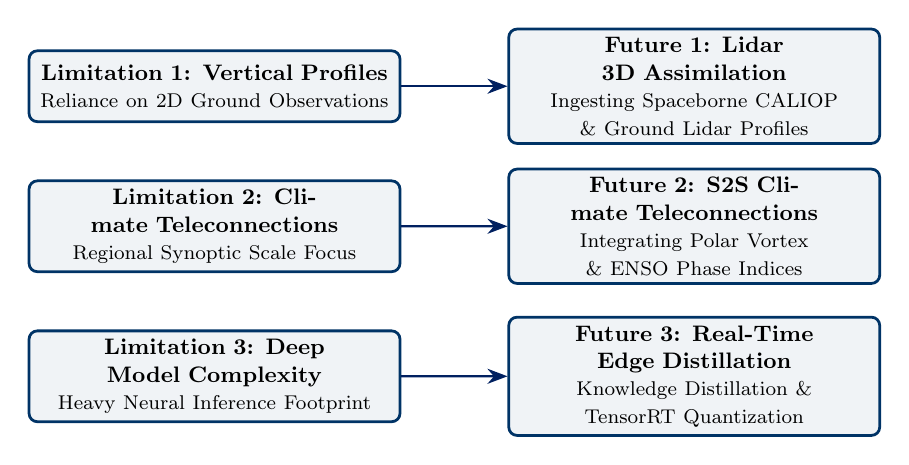
\begin{tikzpicture}[
    scale=0.9, transform shape,
    box/.style={rectangle, draw=ustbblue, fill=ustbblue!6, text centered, rounded corners=3pt, minimum height=1.0cm, line width=1pt, font=\small},
    arrow/.style={-{Stealth[scale=1.1]}, thick, draw=navyblue}
]
\node[box, text width=5.0cm] (l1) {\textbf{Limitation 1: Vertical Profiles}\\ \footnotesize Reliance on 2D Ground Observations};
\node[box, text width=5.0cm, right=1.5cm of l1] (f1) {\textbf{Future 1: Lidar 3D Assimilation}\\ \footnotesize Ingesting Spaceborne CALIOP \& Ground Lidar Profiles};

\node[box, text width=5.0cm, below=0.8cm of l1] (l2) {\textbf{Limitation 2: Climate Teleconnections}\\ \footnotesize Regional Synoptic Scale Focus};
\node[box, text width=5.0cm, right=1.5cm of l2] (f2) {\textbf{Future 2: S2S Climate Teleconnections}\\ \footnotesize Integrating Polar Vortex \& ENSO Phase Indices};

\node[box, text width=5.0cm, below=0.8cm of l2] (l3) {\textbf{Limitation 3: Deep Model Complexity}\\ \footnotesize Heavy Neural Inference Footprint};
\node[box, text width=5.0cm, right=1.5cm of l3] (f3) {\textbf{Future 3: Real-Time Edge Distillation}\\ \footnotesize Knowledge Distillation \& TensorRT Quantization};

\draw[arrow] (l1) -- (f1);
\draw[arrow] (l2) -- (f2);
\draw[arrow] (l3) -- (f3);
\end{tikzpicture}
\caption{Evolutionary Trajectory from Current Limitations to Future Research Directions}
\label{fig:future_directions}
\end{figure}

\begin{enumerate}
    \item \textbf{Vertical Profile Telemetry Constraints and 3D Microphysics}: Current ground networks provide near-surface $\text{PM}_{10}$ observations, whereas dust transport frequently occurs within elevated mid-tropospheric layers ($2{,}000\text{--}5{,}000\,\text{m}$). Future work should assimilate spaceborne lidar (CALIPSO/CALIOP, EarthCARE) and ground-based micro-pulse lidar (MPL) extinction profiles to upgrade the 2D surface model into a full 3D volumetric spatiotemporal assimilation engine.
    \item \textbf{Cross-Scale Planetary Teleconnections and S2S Forecasting}: Sandstorm activity is modulated by sub-seasonal to seasonal (S2S) climate drivers, including Arctic Oscillation (AO) phase shifts, Siberian High anomalies, and El Ni\~no-Southern Oscillation (ENSO) teleconnections. Incorporating hemispheric planetary wave indices into feature stores represents a promising pathway for extending forecasting horizons toward monthly and seasonal outlooks.
    \item \textbf{Model Compression and Real-Time Edge Inference}: Full execution of the deep ST-GNN and AI-GAMFS foundation layers requires substantial GPU compute. Future developments should explore knowledge distillation, weight pruning, and TensorRT INT8 quantization to enable sub-second edge inference on embedded devices, supporting real-time emergency dispatch across intelligent transportation networks and municipal command centers.
\end{enumerate}

---

\section{Chapter Summary}
\label{sec:ch7_summary}

This final chapter synthesized the primary conclusions, academic innovations, engineering applications, and future research trajectories of this dissertation. The proposed \textbf{DustML} architecture demonstrates that coupling physical first principles with deep spatiotemporal graphs effectively overcomes the classical trade-off between numerical physical consistency and machine learning empirical precision, providing a transformative technological foundation for regional disaster prevention and atmospheric environmental protection in East Asia.


% Back Matter
\backmatter

% --- Bibliography ---
\cleardoublepage
\addcontentsline{toc}{chapter}{References}
\bibliography{references}

\end{document}
